\section{Camera Calibration and 3d Reconstruction}

The functions in this section use the so-called pinhole camera model. That
is, a scene view is formed by projecting 3D points into the image plane
using a perspective transformation.

\[
s \; m' = A [R|t] M'
\]

or

\[
s \vecthree{u}{v}{1} = \vecthreethree
{f_x}{0}{c_x}
{0}{f_y}{c_y}
{0}{0}{1}
\begin{bmatrix}
 r_{11} & r_{12} & r_{13} & t_1 \\
 r_{21} & r_{22} & r_{23} & t_2 \\
 r_{31} & r_{32} & r_{33} & t_3
\end{bmatrix}
\begin{bmatrix}X\\Y\\Z\\1 \end{bmatrix}
\]

Where $(X, Y, Z)$ are the coordinates of a 3D point in the world
coordinate space, $(u, v)$ are the coordinates of the projection point
in pixels. $A$ is called a camera matrix, or a matrix of
intrinsic parameters. $(cx, cy)$ is a principal point (that is
usually at the image center), and $fx, fy$ are the focal lengths
expressed in pixel-related units. Thus, if an image from camera is
scaled by some factor, all of these parameters should
be scaled (multiplied/divided, respectively) by the same factor. The
matrix of intrinsic parameters does not depend on the scene viewed and,
once estimated, can be re-used (as long as the focal length is fixed (in
case of zoom lens)). The joint rotation-translation matrix $[R|t]$
is called a matrix of extrinsic parameters. It is used to describe the
camera motion around a static scene, or vice versa, rigid motion of an
object in front of still camera. That is, $[R|t]$ translates
coordinates of a point $(X, Y, Z)$ to some coordinate system,
fixed with respect to the camera. The transformation above is equivalent
to the following (when $z \ne 0$):

\[
\begin{array}{l}
\vecthree{x}{y}{z} = R \vecthree{X}{Y}{Z} + t\\
x' = x/z\\
y' = y/z\\
u = f_x*x' + c_x\\
v = f_y*y' + c_y
\end{array}
\]

Real lenses usually have some distortion, mostly
radial distortion and slight tangential distortion. So, the above model
is extended as:

\[
\begin{array}{l}
\vecthree{x}{y}{z} = R \vecthree{X}{Y}{Z} + t\\
x' = x/z\\
y' = y/z\\
x'' = x' \frac{1 + k_1 r^2 + k_2 r^4 + k_3 r^6}{1 + k_4 r^2 + k_5 r^4 + k_6 r^6} + 2 p_1 x' y' + p_2(r^2 + 2 x'^2) \\
y'' = y' \frac{1 + k_1 r^2 + k_2 r^4 + k_3 r^6}{1 + k_4 r^2 + k_5 r^4 + k_6 r^6} + p_1 (r^2 + 2 y'^2) + 2 p_2 x' y' \\
\text{where} \quad r^2 = x'^2 + y'^2 \\
u = f_x*x'' + c_x\\
v = f_y*y'' + c_y
\end{array}
\]

$k_1$, $k_2$, $k_3$, $k_4$, $k_5$, $k_6$ are radial distortion coefficients, $p_1$, $p_2$ are tangential distortion coefficients.
Higher-order coefficients are not considered in OpenCV. In the functions below the coefficients are passed or returned as
\[ (k_1, k_2, p_1, p_2[, k_3[, k_4, k_5, k_6]]) \] vector. That is, if the vector contains 4 elements, it means that $k_3=0$.
The distortion coefficients do not depend on the scene viewed, thus they also belong to the intrinsic camera parameters.
\emph{And they remain the same regardless of the captured image resolution.}
That is, if, for example, a camera has been calibrated on images of $320
\times 240$ resolution, absolutely the same distortion coefficients can
be used for images of $640 \times 480$ resolution from the same camera (while $f_x$,
$f_y$, $c_x$ and $c_y$ need to be scaled appropriately).

The functions below use the above model to

\begin{itemize}
 \item Project 3D points to the image plane given intrinsic and extrinsic parameters
 \item Compute extrinsic parameters given intrinsic parameters, a few 3D points and their projections.
 \item Estimate intrinsic and extrinsic camera parameters from several views of a known calibration pattern (i.e. every view is described by several 3D-2D point correspondences).
 \item Estimate the relative position and orientation of the stereo camera "heads" and compute the \emph{rectification} transformation that makes the camera optical axes parallel.
\end{itemize}

\ifC

\cvCPyFunc{CalcImageHomography}
Calculates the homography matrix for an oblong planar object (e.g. arm).

\cvdefC{
void cvCalcImageHomography( \par float* line,\par CvPoint3D32f* center,\par float* intrinsic,\par float* homography );
}
\cvdefPy{CalcImageHomography(line,center)-> (intrinsic,homography)}

\begin{description}
\cvarg{line}{the main object axis direction (vector (dx,dy,dz))}
\cvarg{center}{object center ((cx,cy,cz))}
\cvarg{intrinsic}{intrinsic camera parameters (3x3 matrix)}
\cvarg{homography}{output homography matrix (3x3)}
\end{description}

The function calculates the homography
matrix for the initial image transformation from image plane to the
plane, defined by a 3D oblong object line (See \_\_Figure 6-10\_\_
in the OpenCV Guide 3D Reconstruction Chapter).

\fi

\ifCPy
\cvCPyFunc{CalibrateCamera2}
\else
\cvCppFunc{calibrateCamera}
\fi
Finds the camera intrinsic and extrinsic parameters from several views of a calibration pattern.

\cvdefC{double cvCalibrateCamera2( \par const CvMat* objectPoints,\par const CvMat* imagePoints,\par const CvMat* pointCounts,\par CvSize imageSize,\par CvMat* cameraMatrix,\par CvMat* distCoeffs,\par CvMat* rvecs=NULL,\par CvMat* tvecs=NULL,\par int flags=0 );}
\cvdefPy{CalibrateCamera2(objectPoints,imagePoints,pointCounts,imageSize,cameraMatrix,distCoeffs,rvecs,tvecs,flags=0)-> None}
\cvdefCpp{double calibrateCamera( const vector<vector<Point3f> >\& objectPoints,\par
                      const vector<vector<Point2f> >\& imagePoints,\par
                      Size imageSize,\par
                      Mat\& cameraMatrix, Mat\& distCoeffs,\par
                      vector<Mat>\& rvecs, vector<Mat>\& tvecs,\par
                      int flags=0 );}
\begin{description}
\ifCPy
\cvarg{objectPoints}{The joint matrix of object points - calibration pattern features in the model coordinate space. It is floating-point 3xN or Nx3 1-channel, or 1xN or Nx1 3-channel array, where N is the total number of points in all views.}
\cvarg{imagePoints}{The joint matrix of object points projections in the camera views. It is floating-point 2xN or Nx2 1-channel, or 1xN or Nx1 2-channel array, where N is the total number of points in all views}
\cvarg{pointCounts}{Integer 1xM or Mx1 vector (where M is the number of calibration pattern views) containing the number of points in each particular view. The sum of vector elements must match the size of \texttt{objectPoints} and \texttt{imagePoints} (=N).}
\fi
\ifCpp
\cvarg{objectPoints}{The vector of vectors of points on the calibration pattern in its coordinate system, one vector per view. If the same calibration pattern is shown in each view and it's fully visible then all the vectors will be the same, although it is possible to use partially occluded patterns, or even different patterns in different views - then the vectors will be different. The points are 3D, but since they are in the pattern coordinate system, then if the rig is planar, it may have sense to put the model to the XY coordinate plane, so that Z-coordinate of each input object point is 0}
\cvarg{imagePoints}{The vector of vectors of the object point projections on the calibration pattern views, one vector per a view. The projections must be in the same order as the corresponding object points.}
\fi
\cvarg{imageSize}{Size of the image, used only to initialize the intrinsic camera matrix}
\cvarg{cameraMatrix}{The output 3x3 floating-point camera matrix $A = \vecthreethree{f_x}{0}{c_x}{0}{f_y}{c_y}{0}{0}{1}$.\newline
If \texttt{CV\_CALIB\_USE\_INTRINSIC\_GUESS} and/or \texttt{CV\_CALIB\_FIX\_ASPECT\_RATIO} are specified, some or all of \texttt{fx, fy, cx, cy} must be initialized before calling the function}
\cvarg{distCoeffs}{The output vector of distortion coefficients $(k_1, k_2, p_1, p_2[, k_3[, k_4, k_5, k_6]])$ of 4, 5 or 8 elements}
\cvarg{rvecs}{The output \cvCPy{3x\emph{M} or \emph{M}x3 1-channel, or 1x\emph{M} or \emph{M}x1 3-channel array}\cvCpp{vector} of rotation vectors (see \cvCross{Rodrigues2}{Rodrigues}), estimated for each pattern view. That is, each k-th rotation vector together with the corresponding k-th translation vector (see the next output parameter description) brings the calibration pattern from the model coordinate space (in which object points are specified) to the world coordinate space, i.e. real position of the calibration pattern in the k-th pattern view (k=0..\emph{M}-1)}
\cvarg{tvecs}{The output \cvCPy{3x\emph{M} or \emph{M}x3 1-channel, or 1x\emph{M} or \emph{M}x1 3-channel array}\cvCpp{vector} of translation vectors, estimated for each pattern view.}
\cvarg{flags}{Different flags, may be 0 or combination of the following values:
\begin{description}
\cvarg{CV\_CALIB\_USE\_INTRINSIC\_GUESS}{\texttt{cameraMatrix} contains the valid initial values of \texttt{fx, fy, cx, cy} that are optimized further. Otherwise, \texttt{(cx, cy)} is initially set to the image center (\texttt{imageSize} is used here), and focal distances are computed in some least-squares fashion. Note, that if intrinsic parameters are known, there is no need to use this function just to estimate the extrinsic parameters. Use \cvCross{FindExtrinsicCameraParams2}{solvePnP} instead.}
\cvarg{CV\_CALIB\_FIX\_PRINCIPAL\_POINT}{The principal point is not changed during the global optimization, it stays at the center or at the other location specified when \newline \texttt{CV\_CALIB\_USE\_INTRINSIC\_GUESS} is set too.}
\cvarg{CV\_CALIB\_FIX\_ASPECT\_RATIO}{The functions considers only \texttt{fy} as a free parameter, the ratio \texttt{fx/fy} stays the same as in the input \texttt{cameraMatrix}. \newline When \texttt{CV\_CALIB\_USE\_INTRINSIC\_GUESS} is not set, the actual input values of \texttt{fx} and \texttt{fy} are ignored, only their ratio is computed and used further.}
\cvarg{CV\_CALIB\_ZERO\_TANGENT\_DIST}{Tangential distortion coefficients $(p_1, p_2)$ will be set to zeros and stay zero.}}
\cvarg{CV\_CALIB\_FIX\_K1,...,CV\_CALIB\_FIX\_K6}{Do not change the corresponding radial distortion coefficient during the optimization. If \texttt{CV\_CALIB\_USE\_INTRINSIC\_GUESS} is set, the coefficient from the supplied \texttt{distCoeffs} matrix is used, otherwise it is set to 0.}
\cvarg{CV\_CALIB\_RATIONAL\_MODEL}{Enable coefficients k4, k5 and k6. To provide the backward compatibility, this extra flag should be explicitly specified to make the calibration function use the rational model and return 8 coefficients. If the flag is not set, the function will compute \cvCpp{and return} only 5 distortion coefficients.}
\end{description}
\end{description}

The function estimates the intrinsic camera
parameters and extrinsic parameters for each of the views. The
coordinates of 3D object points and their correspondent 2D projections
in each view must be specified. That may be achieved by using an
object with known geometry and easily detectable feature points.
Such an object is called a calibration rig or calibration pattern,
and OpenCV has built-in support for a chessboard as a calibration
rig (see \cvCross{FindChessboardCorners}{findChessboardCorners}). Currently, initialization
of intrinsic parameters (when \texttt{CV\_CALIB\_USE\_INTRINSIC\_GUESS}
is not set) is only implemented for planar calibration patterns
(where z-coordinates of the object points must be all 0's). 3D
calibration rigs can also be used as long as initial \texttt{cameraMatrix}
is provided.

The algorithm does the following:
\begin{enumerate}
    \item First, it computes the initial intrinsic parameters (the option only available for planar calibration patterns) or reads them from the input parameters. The distortion coefficients are all set to zeros initially (unless some of \texttt{CV\_CALIB\_FIX\_K?} are specified).
    \item The initial camera pose is estimated as if the intrinsic parameters have been already known. This is done using \cvCross{FindExtrinsicCameraParams2}{solvePnP}
    \item After that the global Levenberg-Marquardt optimization algorithm is run to minimize the reprojection error, i.e. the total sum of squared distances between the observed feature points \texttt{imagePoints} and the projected (using the current estimates for camera parameters and the poses) object points \texttt{objectPoints}; see \cvCross{ProjectPoints2}{projectPoints}.
\end{enumerate}

\ifPy
\else
The function returns the final re-projection error.
\fi

Note: if you're using a non-square (=non-NxN) grid and
\cvCppCross{findChessboardCorners} for calibration, and \texttt{calibrateCamera} returns
bad values (i.e. zero distortion coefficients, an image center very far from
$(w/2-0.5,h/2-0.5)$, and / or large differences between $f_x$ and $f_y$ (ratios of
10:1 or more)), then you've probably used \texttt{patternSize=cvSize(rows,cols)},
but should use \texttt{patternSize=cvSize(cols,rows)} in \cvCross{FindChessboardCorners}{findChessboardCorners}.

See also: \cvCross{FindChessboardCorners}{findChessboardCorners}, \cvCross{FindExtrinsicCameraParams2}{solvePnP}, \cvCppCross{initCameraMatrix2D}, \cvCross{StereoCalibrate}{stereoCalibrate}, \cvCross{Undistort2}{undistort}

\ifCpp

\cvCppFunc{calibrationMatrixValues}
Computes some useful camera characteristics from the camera matrix

\cvdefCpp{void calibrationMatrixValues( const Mat\& cameraMatrix,\par
                              Size imageSize,\par
                              double apertureWidth,\par
                              double apertureHeight,\par
                              double\& fovx,\par
                              double\& fovy,\par
                              double\& focalLength,\par
                              Point2d\& principalPoint,\par
                              double\& aspectRatio );}
\begin{description}
\cvarg{cameraMatrix}{The input camera matrix that can be estimated by \cvCppCross{calibrateCamera} or \cvCppCross{stereoCalibrate}}
\cvarg{imageSize}{The input image size in pixels}
\cvarg{apertureWidth}{Physical width of the sensor}
\cvarg{apertureHeight}{Physical height of the sensor}
\cvarg{fovx}{The output field of view in degrees along the horizontal sensor axis}
\cvarg{fovy}{The output field of view in degrees along the vertical sensor axis}
\cvarg{focalLength}{The focal length of the lens in mm}
\cvarg{principalPoint}{The principal point in pixels}
\cvarg{aspectRatio}{$f_y/f_x$}
\end{description}

The function computes various useful camera characteristics from the previously estimated camera matrix.

\cvCppFunc{composeRT}
Combines two rotation-and-shift transformations

\cvdefCpp{void composeRT( const Mat\& rvec1, const Mat\& tvec1,\par
                const Mat\& rvec2, const Mat\& tvec2,\par
                Mat\& rvec3, Mat\& tvec3 );\newline
void composeRT( const Mat\& rvec1, const Mat\& tvec1,\par
                const Mat\& rvec2, const Mat\& tvec2,\par
                Mat\& rvec3, Mat\& tvec3,\par
                Mat\& dr3dr1, Mat\& dr3dt1,\par
                Mat\& dr3dr2, Mat\& dr3dt2,\par
                Mat\& dt3dr1, Mat\& dt3dt1,\par
                Mat\& dt3dr2, Mat\& dt3dt2 );}
\begin{description}
\cvarg{rvec1}{The first rotation vector}
\cvarg{tvec1}{The first translation vector}
\cvarg{rvec2}{The second rotation vector}
\cvarg{tvec2}{The second translation vector}
\cvarg{rvec3}{The output rotation vector of the superposition}
\cvarg{tvec3}{The output translation vector of the superposition}
\cvarg{d??d??}{The optional output derivatives of \texttt{rvec3} or \texttt{tvec3} w.r.t. \texttt{rvec?} or \texttt{tvec?}}
\end{description}

The functions compute:

\[ \begin{array}{l}
\texttt{rvec3} = \mathrm{rodrigues}^{-1}\left(\mathrm{rodrigues}(\texttt{rvec2}) \cdot
\mathrm{rodrigues}(\texttt{rvec1})\right) \\
\texttt{tvec3} = \mathrm{rodrigues}(\texttt{rvec2}) \cdot \texttt{tvec1} + \texttt{tvec2}
\end{array}, \]

where $\mathrm{rodrigues}$ denotes a rotation vector to rotation matrix transformation, and $\mathrm{rodrigues}^{-1}$ denotes the inverse transformation, see \cvCppCross{Rodrigues}.

Also, the functions can compute the derivatives of the output vectors w.r.t the input vectors (see \cvCppCross{matMulDeriv}).
The functions are used inside \cvCppCross{stereoCalibrate} but can also be used in your own code where Levenberg-Marquardt or another gradient-based solver is used to optimize a function that contains matrix multiplication.

\fi

\ifCPy
\cvCPyFunc{ComputeCorrespondEpilines}
\else
\cvCppFunc{computeCorrespondEpilines}
\fi
For points in one image of a stereo pair, computes the corresponding epilines in the other image.

\cvdefC{void cvComputeCorrespondEpilines( \par const CvMat* points,\par int whichImage,\par const CvMat* F, \par CvMat* lines);}
\cvdefPy{ComputeCorrespondEpilines(points, whichImage, F, lines) -> None}
\cvdefCpp{void computeCorrespondEpilines( const Mat\& points,\par
                                int whichImage, const Mat\& F,\par
                                vector<Vec3f>\& lines );}
\begin{description}
\cvCPy{\cvarg{points}{The input points. \texttt{2xN, Nx2, 3xN} or \texttt{Nx3} array (where \texttt{N} number of points). Multi-channel \texttt{1xN} or \texttt{Nx1} array is also acceptable}}
\cvCpp{\cvarg{points}{The input points. $N \times 1$ or $1 \times N$ matrix of type \texttt{CV\_32FC2} or \texttt{vector<Point2f>}}}
\cvarg{whichImage}{Index of the image (1 or 2) that contains the \texttt{points}}
\cvarg{F}{The fundamental matrix that can be estimated using \cvCross{FindFundamentalMat}{findFundamentalMat}
or \cvCross{StereoRectify}{stereoRectify}.}
\cvarg{lines}{\cvCPy{The output epilines, a \texttt{3xN} or \texttt{Nx3} array.}\cvCpp{The output vector of the corresponding to the points epipolar lines in the other image.} Each line $ax + by + c=0$ is encoded by 3 numbers $(a, b, c)$}
\end{description}

For every point in one of the two images of a stereo-pair the function finds the equation of the
corresponding epipolar line in the other image.

From the fundamental matrix definition (see \cvCross{FindFundamentalMat}{findFundamentalMat}),
line $l^{(2)}_i$ in the second image for the point $p^{(1)}_i$ in the first image (i.e. when \texttt{whichImage=1}) is computed as:

\[ l^{(2)}_i = F p^{(1)}_i \]

and, vice versa, when \texttt{whichImage=2}, $l^{(1)}_i$ is computed from $p^{(2)}_i$ as:

\[ l^{(1)}_i = F^T p^{(2)}_i \]

Line coefficients are defined up to a scale. They are normalized, such that $a_i^2+b_i^2=1$.

\ifCPy
\cvCPyFunc{ConvertPointsHomogeneous}
\else
\cvCppFunc{convertPointsHomogeneous}
\fi
Convert points to/from homogeneous coordinates.

\cvdefC{void cvConvertPointsHomogeneous( \par const CvMat* src,\par CvMat* dst );}

\cvdefPy{ConvertPointsHomogeneous( src, dst ) -> None}

\cvdefCpp{void convertPointsHomogeneous( const Mat\& src, vector<Point3f>\& dst );\newline
void convertPointsHomogeneous( const Mat\& src, vector<Point2f>\& dst );}

\begin{description}
\ifC
\cvarg{src}{The input point array, \texttt{2xN, Nx2, 3xN, Nx3, 4xN or Nx4 (where \texttt{N} is the number of points)}. Multi-channel \texttt{1xN} or \texttt{Nx1} array is also acceptable}
\cvarg{dst}{The output point array, must contain the same number of points as the input; The dimensionality must be the same, 1 less or 1 more than the input, and also within 2 to 4}
\else
\cvarg{src}{The input array or vector of 2D, 3D or 4D points}
\cvarg{dst}{The output vector of 2D or 2D points}
\fi
\end{description}

The \cvC{function converts}\cvCpp{functions convert} 2D or 3D points from/to homogeneous coordinates, or simply \cvC{copies or transposes}\cvCpp{copy or transpose} the array. If the input array dimensionality is larger than the output, each coordinate is divided by the last coordinate:

\[
\begin{array}{l}
(x,y[,z],w) -> (x',y'[,z'])\\
\text{where} \\
x' = x/w \\
y' = y/w \\
z' = z/w \quad \text{(if output is 3D)}
\end{array}
\]

If the output array dimensionality is larger, an extra 1 is appended to each point.  Otherwise, the input array is simply copied (with optional transposition) to the output.

\cvC{\textbf{Note} because the function accepts a large variety of array layouts, it may report an error when input/output array dimensionality is ambiguous. It is always safe to use the function with number of points $\texttt{N} \ge 5$, or to use multi-channel \texttt{Nx1} or \texttt{1xN} arrays.}

\ifCPy

\cvCPyFunc{CreatePOSITObject}
Initializes a structure containing object information.

\cvdefC{
CvPOSITObject* cvCreatePOSITObject( \par CvPoint3D32f* points,\par int point\_count );
}\cvdefPy{CreatePOSITObject(points)-> POSITObject}

\begin{description}
\ifC
\cvarg{points}{Pointer to the points of the 3D object model}
\cvarg{point\_count}{Number of object points}
\else
\cvarg{points}{List of 3D points}
\fi
\end{description}

The function allocates memory for the object structure and computes the object inverse matrix.

The preprocessed object data is stored in the structure \cvCPyCross{CvPOSITObject}, internal for OpenCV, which means that the user cannot directly access the structure data. The user may only create this structure and pass its pointer to the function.

An object is defined as a set of points given in a coordinate system. The function \cvCPyCross{POSIT} computes a vector that begins at a camera-related coordinate system center and ends at the \texttt{points[0]} of the object.

Once the work with a given object is finished, the function \cvCPyCross{ReleasePOSITObject} must be called to free memory.

\cvCPyFunc{CreateStereoBMState}
Creates block matching stereo correspondence structure.

\cvdefC{

CvStereoBMState* cvCreateStereoBMState( int preset=CV\_STEREO\_BM\_BASIC,
                                        int numberOfDisparities=0 );

}
\cvdefPy{CreateStereoBMState(preset=CV\_STEREO\_BM\_BASIC,numberOfDisparities=0)-> StereoBMState}

\begin{description}
\cvarg{preset}{ID of one of the pre-defined parameter sets. Any of the parameters can be overridden after creating the structure.  Values are
\begin{description}
\cvarg{CV\_STEREO\_BM\_BASIC}{Parameters suitable for general cameras}
\cvarg{CV\_STEREO\_BM\_FISH\_EYE}{Parameters suitable for wide-angle cameras}
\cvarg{CV\_STEREO\_BM\_NARROW}{Parameters suitable for narrow-angle cameras}
\end{description}
}
\cvarg{numberOfDisparities}{The number of disparities. If the parameter is 0, it is taken from the preset, otherwise the supplied value overrides the one from preset.}
\end{description}

The function creates the stereo correspondence structure and initializes
it. It is possible to override any of the parameters at any time between
the calls to \cvCPyCross{FindStereoCorrespondenceBM}.

\cvCPyFunc{CreateStereoGCState}
Creates the state of graph cut-based stereo correspondence algorithm.

\cvdefC{

CvStereoGCState* cvCreateStereoGCState( int numberOfDisparities,
                                        int maxIters );

}
\cvdefPy{CreateStereoGCState(numberOfDisparities,maxIters)-> StereoGCState}

\begin{description}
\cvarg{numberOfDisparities}{The number of disparities. The disparity search range will be $\texttt{state->minDisparity} \le disparity < \texttt{state->minDisparity} + \texttt{state->numberOfDisparities}$}
\cvarg{maxIters}{Maximum number of iterations. On each iteration all possible (or reasonable) alpha-expansions are tried. The algorithm may terminate earlier if it could not find an alpha-expansion that decreases the overall cost function value. See \cite{Kolmogorov03}  for details. }
\end{description}

The function creates the stereo correspondence structure and initializes it. It is possible to override any of the parameters at any time between the calls to \cvCPyCross{FindStereoCorrespondenceGC}.

\cvclass{CvStereoBMState}
The structure for block matching stereo correspondence algorithm.

\ifC
\begin{lstlisting}
typedef struct CvStereoBMState
{
    //pre filters (normalize input images):
    int       preFilterType; // 0 for now
    int       preFilterSize; // ~5x5..21x21
    int       preFilterCap;  // up to ~31
    //correspondence using Sum of Absolute Difference (SAD):
    int       SADWindowSize; // Could be 5x5..21x21
    int       minDisparity;  // minimum disparity (=0)
    int       numberOfDisparities; // maximum disparity - minimum disparity
    //post filters (knock out bad matches):
    int       textureThreshold; // areas with no texture are ignored
    int       uniquenessRatio;// invalidate disparity at pixels where there are other close matches
                              // with different disparity
    int       speckleWindowSize; // the maximum area of speckles to remove
                                 // (set to 0 to disable speckle filtering)
    int       speckleRange; // acceptable range of disparity variation in each connected component
    
    int trySmallerWindows; // not used 
    CvRect roi1, roi2; // clipping ROIs
    
    int disp12MaxDiff; // maximum allowed disparity difference in the left-right check 
    
    // internal data
    ...
}
CvStereoBMState;
\end{lstlisting}
\fi
\begin{description}
\cvarg{preFilterType}{type of the prefilter, \texttt{CV\_STEREO\_BM\_NORMALIZED\_RESPONSE} or the default and the recommended \texttt{CV\_STEREO\_BM\_XSOBEL}, int}
\cvarg{preFilterSize}{~5x5..21x21, int}
\cvarg{preFilterCap}{up to ~31, int}
\cvarg{SADWindowSize}{Could be 5x5..21x21 or higher, but with 21x21 or smaller windows the processing speed is much higher, int}
\cvarg{minDisparity}{minimum disparity (=0), int}
\cvarg{numberOfDisparities}{maximum disparity - minimum disparity, int}
\cvarg{textureThreshold}{the textureness threshold. That is, if the sum of absolute values of x-derivatives computed over \texttt{SADWindowSize} by \texttt{SADWindowSize} pixel neighborhood is smaller than the parameter, no disparity is computed at the pixel, int}
\cvarg{uniquenessRatio}{the minimum margin in percents between the best (minimum) cost function value and the second best value to accept the computed disparity, int}
\cvarg{speckleWindowSize}{the maximum area of speckles to remove (set to 0 to disable speckle filtering), int}
\cvarg{speckleRange}{acceptable range of disparity variation in each connected component, int}
\cvarg{trySmallerWindows}{not used currently (0), int}
\cvarg{roi1, roi2}{These are the clipping ROIs for the left and the right images. The function \cvCPyCross{StereoRectify} returns the largest rectangles in the left and right images where after the rectification all the pixels are valid. If you copy those rectangles to the \texttt{CvStereoBMState} structure, the stereo correspondence function will automatically clear out the pixels outside of the "valid" disparity rectangle computed by \cvCPyCross{GetValidDisparityROI}. Thus you will get more "invalid disparity" pixels than usual, but the remaining pixels are more probable to be valid.}
\cvarg{disp12MaxDiff}{The maximum allowed difference between the explicitly computed left-to-right disparity map and the implicitly (by \cvCPyCross{ValidateDisparity}) computed right-to-left disparity. If for some pixel the difference is larger than the specified threshold, the disparity at the pixel is invalidated. By default this parameter is set to (-1), which means that the left-right check is not performed.}
\end{description}


The block matching stereo correspondence algorithm, by Kurt Konolige, is very fast single-pass stereo matching algorithm that uses sliding sums of absolute differences between pixels in the left image and the pixels in the right image, shifted by some varying amount of pixels (from \texttt{minDisparity} to \texttt{minDisparity+numberOfDisparities}). On a pair of images WxH the algorithm computes disparity in \texttt{O(W*H*numberOfDisparities)} time. In order to improve quality and readability of the disparity map, the algorithm includes pre-filtering and post-filtering procedures.

Note that the algorithm searches for the corresponding blocks in x direction only. It means that the supplied stereo pair should be rectified. Vertical stereo layout is not directly supported, but in such a case the images could be transposed by user.

\cvclass{CvStereoGCState}
The structure for graph cuts-based stereo correspondence algorithm

\ifC
\begin{lstlisting}
typedef struct CvStereoGCState
{
    int Ithreshold; // threshold for piece-wise linear data cost function (5 by default)
    int interactionRadius; // radius for smoothness cost function (1 by default; means Potts model)
    float K, lambda, lambda1, lambda2; // parameters for the cost function
                                       // (usually computed adaptively from the input data)
    int occlusionCost; // 10000 by default
    int minDisparity; // 0 by default; see CvStereoBMState
    int numberOfDisparities; // defined by user; see CvStereoBMState
    int maxIters; // number of iterations; defined by user.

    // internal buffers
    CvMat* left;
    CvMat* right;
    CvMat* dispLeft;
    CvMat* dispRight;
    CvMat* ptrLeft;
    CvMat* ptrRight;
    CvMat* vtxBuf;
    CvMat* edgeBuf;
}
CvStereoGCState;
\end{lstlisting}
\else
\begin{description}
\cvarg{Ithreshold}{threshold for piece-wise linear data cost function (5 by default)}
\cvarg{interactionRadius}{radius for smoothness cost function (1 by default; means Potts model)}
\cvarg{K, lambda, lambda1, lambda2}{parameters for the cost function (usually computed adaptively from the input data)}
\cvarg{occlusionCost}{10000 by default}
\cvarg{minDisparity}{0 by default; see \cross{CvStereoBMState}}
\cvarg{numberOfDisparities}{defined by user; see \cross{CvStereoBMState}}
\cvarg{maxIters}{number of iterations; defined by user.}
\end{description}
\fi

The graph cuts stereo correspondence algorithm, described in \cite{Kolmogorov03} (as \textbf{KZ1}), is non-realtime stereo correspondence algorithm that usually gives very accurate depth map with well-defined object boundaries. The algorithm represents stereo problem as a sequence of binary optimization problems, each of those is solved using maximum graph flow algorithm. The state structure above should not be allocated and initialized manually; instead, use \cvCPyCross{CreateStereoGCState} and then override necessary parameters if needed.

\fi

\ifCPy
\cvCPyFunc{DecomposeProjectionMatrix}
\else
\cvCppFunc{decomposeProjectionMatrix}
\fi
Decomposes the projection matrix into a rotation matrix and a camera matrix.

\cvdefC{
void cvDecomposeProjectionMatrix( \par const CvMat *projMatrix,\par CvMat *cameraMatrix,\par CvMat *rotMatrix,\par CvMat *transVect,\par CvMat *rotMatrX=NULL,\par CvMat *rotMatrY=NULL,\par CvMat *rotMatrZ=NULL,\par CvPoint3D64f *eulerAngles=NULL);
}

\cvdefPy{DecomposeProjectionMatrix(projMatrix, cameraMatrix, rotMatrix, transVect, rotMatrX = None, rotMatrY = None, rotMatrZ = None) -> eulerAngles}

\cvdefCpp{void decomposeProjectionMatrix( const Mat\& projMatrix,\par
                                Mat\& cameraMatrix,\par
                                Mat\& rotMatrix, Mat\& transVect );\newline
void decomposeProjectionMatrix( const Mat\& projMatrix, \par
                                Mat\& cameraMatrix,\par
                                Mat\& rotMatrix, Mat\& transVect,\par
                                Mat\& rotMatrixX, Mat\& rotMatrixY,\par
                                Mat\& rotMatrixZ, Vec3d\& eulerAngles );}
\begin{description}
\cvarg{projMatrix}{The 3x4 input projection matrix P}
\cvarg{cameraMatrix}{The output 3x3 camera matrix K}
\cvarg{rotMatrix}{The output 3x3 external rotation matrix R}
\cvarg{transVect}{The output 4x1 translation vector T}
\cvarg{rotMatrX}{Optional 3x3 rotation matrix around x-axis}
\cvarg{rotMatrY}{Optional 3x3 rotation matrix around y-axis}
\cvarg{rotMatrZ}{Optional 3x3 rotation matrix around z-axis}
\cvarg{eulerAngles}{Optional 3 points containing the three Euler angles of rotation}
\end{description}

The function computes a decomposition of a projection matrix into a calibration and a rotation matrix and the position of the camera.

It optionally returns three rotation matrices, one for each axis, and the three Euler angles that could be used in OpenGL.

The function is based on \cvCross{RQDecomp3x3}{RQDecomp3x3}.

\ifCPy
\cvCPyFunc{DrawChessboardCorners}
\else
\cvCppFunc{drawChessboardCorners}
\fi
Renders the detected chessboard corners.

\cvdefC{
void cvDrawChessboardCorners( \par CvArr* image,\par CvSize patternSize,\par CvPoint2D32f* corners,\par int count,\par int patternWasFound );
}\cvdefPy{DrawChessboardCorners(image,patternSize,corners,patternWasFound)-> None}
\cvdefCpp{void drawChessboardCorners( Mat\& image, Size patternSize,\par
                            const Mat\& corners,\par
                            bool patternWasFound );}
\begin{description}
\cvarg{image}{The destination image; it must be an 8-bit color image}
\cvarg{patternSize}{The number of inner corners per chessboard row and column. (patternSize = cv::Size(points\_per\_row,points\_per\_column) = cv::Size(rows,columns) )}
\cvarg{corners}{The array of corners detected, this should be the output from findChessboardCorners wrapped in a cv::Mat().}
\cvC{\cvarg{count}{The number of corners}}
\cvarg{patternWasFound}{Indicates whether the complete board was found \cvCPy{$(\ne 0)$} or not \cvCPy{$(=0)$}. One may just pass the return value \cvCPyCross{FindChessboardCorners}{findChessboardCorners} here}
\end{description}

The function draws the individual chessboard corners detected as red circles if the board was not found or as colored corners connected with lines if the board was found.

\ifCPy
\cvCPyFunc{FindChessboardCorners}
\else
\cvCppFunc{findChessboardCorners}
\fi
Finds the positions of the internal corners of the chessboard.

\cvdefC{int cvFindChessboardCorners( \par const void* image,\par CvSize patternSize,\par CvPoint2D32f* corners,\par int* cornerCount=NULL,\par int flags=CV\_CALIB\_CB\_ADAPTIVE\_THRESH );}
\cvdefPy{FindChessboardCorners(image, patternSize, flags=CV\_CALIB\_CB\_ADAPTIVE\_THRESH) -> corners}
\cvdefCpp{bool findChessboardCorners( const Mat\& image, Size patternSize,\par
                            vector<Point2f>\& corners,\par
                            int flags=CV\_CALIB\_CB\_ADAPTIVE\_THRESH+\par
                                 CV\_CALIB\_CB\_NORMALIZE\_IMAGE );}
\begin{description}
\cvarg{image}{Source chessboard view; it must be an 8-bit grayscale or color image}
\cvarg{patternSize}{The number of inner corners per chessboard row and column
( patternSize = cvSize(points\_per\_row,points\_per\_colum) = cvSize(columns,rows) )}
\cvarg{corners}{The output array of corners detected}
\cvC{\cvarg{cornerCount}{The output corner counter. If it is not NULL, it stores the number of corners found}}
\cvarg{flags}{Various operation flags, can be 0 or a combination of the following values:
\begin{description}
 \cvarg{CV\_CALIB\_CB\_ADAPTIVE\_THRESH}{use adaptive thresholding to convert the image to black and white, rather than a fixed threshold level (computed from the average image brightness).}
 \cvarg{CV\_CALIB\_CB\_NORMALIZE\_IMAGE}{normalize the image gamma with \cvCross{EqualizeHist}{equalizeHist} before applying fixed or adaptive thresholding.}
 \cvarg{CV\_CALIB\_CB\_FILTER\_QUADS}{use additional criteria (like contour area, perimeter, square-like shape) to filter out false quads that are extracted at the contour retrieval stage.}
 \cvarg{CALIB\_CB\_FAST\_CHECK}{Runs a fast check on the image that looks for chessboard corners, and shortcuts the call if none are found. This can drastically speed up the call in the degenerate condition when
 no chessboard is observed.}
\end{description}}
\end{description}

The function attempts to determine
whether the input image is a view of the chessboard pattern and
locate the internal chessboard corners. The function returns a non-zero
value if all of the corners have been found and they have been placed
in a certain order (row by row, left to right in every row),
otherwise, if the function fails to find all the corners or reorder
them, it returns 0. For example, a regular chessboard has 8 x 8
squares and 7 x 7 internal corners, that is, points, where the black
squares touch each other. The coordinates detected are approximate,
and to determine their position more accurately, the user may use
the function \cvCross{FindCornerSubPix}{cornerSubPix}.

Sample usage of detecting and drawing chessboard corners:
\begin{lstlisting}
Size patternsize(8,6); //interior number of corners
Mat gray = ....; //source image
vector<Point2f> corners; //this will be filled by the detected corners

//CALIB_CB_FAST_CHECK saves a lot of time on images 
//that don't contain any chessboard corners
bool patternfound = findChessboardCorners(gray, patternsize, corners, 
	CALIB_CB_ADAPTIVE_THRESH + CALIB_CB_NORMALIZE_IMAGE 
	+ CALIB_CB_FAST_CHECK);

if(patternfound)
  cornerSubPix(gray, corners, Size(11, 11), Size(-1, -1), 
    TermCriteria(CV_TERMCRIT_EPS + CV_TERMCRIT_ITER, 30, 0.1));
    
drawChessboardCorners(img, patternsize, Mat(corners), patternfound);
\end{lstlisting}

\textbf{Note:} the function requires some white space (like a square-thick border, the wider the better) around the board to make the detection more robust in various environment (otherwise if there is no border and the background is dark, the outer black squares could not be segmented properly and so the square grouping and ordering algorithm will fail).

\ifCpp
\cvCppFunc{findCirclesGrid}
Finds the centers of the cirlces' grid.
\cvdefCpp{bool findCirclesGrid( const Mat\& image, Size patternSize,\par
                            vector<Point2f>\& centers,\par
                            int flags=0 );}
\begin{description}
\cvarg{image}{Source circles' grid view; it must be an 8-bit grayscale or color
image}
\cvarg{patternSize}{The number of circles per grid row and column
( patternSize = Size( points\_per\_row, points\_per\_colum ) =
Size( columns, rows ) )}
\cvarg{centers}{The output array of centers detected}
\cvarg{flags}{Various operation flags, no flags are supported currently} 
\end{description}

The function attempts to determine
whether the input image is a view of the circles' grid pattern and
locate the circles' centers. The function returns a
non-zero value if all of the centers have been found and they have been placed
in a certain order (row by row, left to right in every row),
otherwise, if the function fails to find all the corners or reorder
them, it returns 0.

Sample usage of detecting and drawing circles' centers:
\begin{lstlisting}
Size patternsize(7,7); //number of centers
Mat gray = ....; //source image
vector<Point2f> centers; //this will be filled by the detected centers

bool patternfound = findCirclesGrid(gray, patternsize, centers);
    
drawChessboardCorners(img, patternsize, Mat(centers), patternfound);
\end{lstlisting}

\textbf{Note:} the function requires some white space (like a square-thick border, the wider the better) around the board to make the detection more robust in various environment.
\fi

\ifCPy
\cvCPyFunc{FindExtrinsicCameraParams2}
\else
\cvCppFunc{solvePnP}
\fi
Finds the object pose from the 3D-2D point correspondences

\cvdefC{void cvFindExtrinsicCameraParams2( \par const CvMat* objectPoints,\par const CvMat* imagePoints,\par const CvMat* cameraMatrix,\par const CvMat* distCoeffs,\par CvMat* rvec,\par CvMat* tvec, \par int useExtrinsicGuess=0);}
\cvdefPy{FindExtrinsicCameraParams2(objectPoints,imagePoints,cameraMatrix,distCoeffs,rvec,tvec,useExtrinsicGuess=0)-> None}
\cvdefCpp{void solvePnP( const Mat\& objectPoints,\par
               const Mat\& imagePoints,\par
               const Mat\& cameraMatrix,\par
               const Mat\& distCoeffs,\par
               Mat\& rvec, Mat\& tvec,\par
               bool useExtrinsicGuess=false );}
\begin{description}
\cvarg{objectPoints}{The array of object points in the object coordinate space, 3xN or Nx3 1-channel, or 1xN or Nx1 3-channel, where N is the number of points. \cvCpp{Can also pass \texttt{vector<Point3f>} here.}}
\cvarg{imagePoints}{The array of corresponding image points, 2xN or Nx2 1-channel or 1xN or Nx1 2-channel, where N is the number of points. \cvCpp{Can also pass \texttt{vector<Point2f>} here.}}
\cvarg{cameraMatrix}{The input camera matrix $A = \vecthreethree{fx}{0}{cx}{0}{fy}{cy}{0}{0}{1} $}
\cvarg{distCoeffs}{The input vector of distortion coefficients $(k_1, k_2, p_1, p_2[, k_3[, k_4, k_5, k_6]])$ of 4, 5 or 8 elements. If the vector is NULL/empty, the zero distortion coefficients are assumed.}
\cvarg{rvec}{The output rotation vector (see \cvCross{Rodrigues2}{Rodrigues}) that (together with \texttt{tvec}) brings points from the model coordinate system to the camera coordinate system}
\cvarg{tvec}{The output translation vector}
\cvarg{useExtrinsicGuess}{If true (1), the function will use the provided \texttt{rvec} and \texttt{tvec} as the initial approximations of the rotation and translation vectors, respectively, and will further optimize them.}
\end{description}

The function estimates the object pose given a set of object points, their corresponding image projections, as well as the camera matrix and the distortion coefficients. This function finds such a pose that minimizes reprojection error, i.e. the sum of squared distances between the observed projections \texttt{imagePoints} and the projected (using \cvCross{ProjectPoints2}{projectPoints}) \texttt{objectPoints}.


\ifCPy
The function's counterpart in the C++ API is \hyperref[cppfunc.solvePnP]{cv::solvePnP}
\fi

\ifCPy
\cvCPyFunc{FindFundamentalMat}
\else
\cvCppFunc{findFundamentalMat}
\fi

Calculates the fundamental matrix from the corresponding points in two images.

\cvdefC{
int cvFindFundamentalMat( \par const CvMat* points1,\par const CvMat* points2,\par CvMat* fundamentalMatrix,\par int    method=CV\_FM\_RANSAC,\par double param1=1.,\par double param2=0.99,\par CvMat* status=NULL);
}
\cvdefPy{FindFundamentalMat(points1, points2, fundamentalMatrix, method=CV\_FM\_RANSAC, param1=1., param2=0.99, status = None) -> None}
\cvdefCpp{Mat findFundamentalMat( const Mat\& points1, const Mat\& points2,\par
                        vector<uchar>\& status, int method=FM\_RANSAC,\par
                        double param1=3., double param2=0.99 );\newline
Mat findFundamentalMat( const Mat\& points1, const Mat\& points2,\par
                        int method=FM\_RANSAC,\par
                        double param1=3., double param2=0.99 );}
\begin{description}
\cvarg{points1}{Array of \texttt{N} points from the first image.\cvCPy{It can be \texttt{2xN, Nx2, 3xN} or \texttt{Nx3} 1-channel array or  \texttt{1xN} or \texttt{Nx1} 2- or 3-channel array}. The point coordinates should be floating-point (single or double precision)}
\cvarg{points2}{Array of the second image points of the same size and format as \texttt{points1}}
\cvCPy{\cvarg{fundamentalMatrix}{The output fundamental matrix or matrices. The size should be 3x3 or 9x3 (7-point method may return up to 3 matrices)}}
\cvarg{method}{Method for computing the fundamental matrix
\begin{description}
  \cvarg{CV\_FM\_7POINT}{for a 7-point algorithm. $N = 7$}
  \cvarg{CV\_FM\_8POINT}{for an 8-point algorithm. $N \ge 8$}
  \cvarg{CV\_FM\_RANSAC}{for the RANSAC algorithm. $N \ge 8$}
  \cvarg{CV\_FM\_LMEDS}{for the LMedS algorithm. $N \ge 8$}
\end{description}}
\cvarg{param1}{The parameter is used for RANSAC. It is the maximum distance from point to epipolar line in pixels, beyond which the point is considered an outlier and is not used for computing the final fundamental matrix. It can be set to something like 1-3, depending on the accuracy of the point localization, image resolution and the image noise}
\cvarg{param2}{The parameter is used for RANSAC or LMedS methods only. It specifies the desirable level of confidence (probability) that the estimated matrix is correct}
\cvarg{status}{The \cvCPy{optional} output array of N elements, every element of which is set to 0 for outliers and to 1 for the other points. The array is computed only in RANSAC and LMedS methods. For other methods it is set to all 1's}
\end{description}

The epipolar geometry is described by the following equation:

\[ [p_2; 1]^T F [p_1; 1] = 0 \]

where $F$ is fundamental matrix, $p_1$ and $p_2$ are corresponding points in the first and the second images, respectively.

The function calculates the fundamental matrix using one of four methods listed above and returns \cvCpp{the found fundamental matrix}\cvCPy{the number of fundamental matrices found (1 or 3) and 0, if no matrix is found}. Normally just 1 matrix is found, but in the case of 7-point algorithm the function may return up to 3 solutions ($9 \times 3$ matrix that stores all 3 matrices sequentially).

The calculated fundamental matrix may be passed further to
\cvCross{ComputeCorrespondEpilines}{computeCorrespondEpilines} that finds the epipolar lines
corresponding to the specified points. It can also be passed to \cvCross{StereoRectifyUncalibrated}{stereoRectifyUncalibrated} to compute the rectification transformation.

\ifC
% Example. Estimation of fundamental matrix using RANSAC algorithm
\begin{lstlisting}
int point_count = 100;
CvMat* points1;
CvMat* points2;
CvMat* status;
CvMat* fundamental_matrix;

points1 = cvCreateMat(1,point_count,CV_32FC2);
points2 = cvCreateMat(1,point_count,CV_32FC2);
status = cvCreateMat(1,point_count,CV_8UC1);

/* Fill the points here ... */
for( i = 0; i < point_count; i++ )
{
    points1->data.fl[i*2] = <x,,1,i,,>;
    points1->data.fl[i*2+1] = <y,,1,i,,>;
    points2->data.fl[i*2] = <x,,2,i,,>;
    points2->data.fl[i*2+1] = <y,,2,i,,>;
}

fundamental_matrix = cvCreateMat(3,3,CV_32FC1);
int fm_count = cvFindFundamentalMat( points1,points2,fundamental_matrix,
                                     CV_FM_RANSAC,1.0,0.99,status );
\end{lstlisting}
\fi
\ifCpp
\begin{lstlisting}
// Example. Estimation of fundamental matrix using RANSAC algorithm
int point_count = 100;
vector<Point2f> points1(point_count);
vector<Point2f> points2(point_count);

// initialize the points here ... */
for( int i = 0; i < point_count; i++ )
{
    points1[i] = ...;
    points2[i] = ...;
}

Mat fundamental_matrix =
 findFundamentalMat(points1, points2, FM_RANSAC, 3, 0.99);
\end{lstlisting}
\fi

\ifCPy
\cvCPyFunc{FindHomography}
\else
\cvCppFunc{findHomography}
\fi
Finds the perspective transformation between two planes.

\cvdefC{void cvFindHomography( \par const CvMat* srcPoints,\par const CvMat* dstPoints,\par CvMat* H \par
int method=0, \par double ransacReprojThreshold=3, \par CvMat* status=NULL);}
\cvdefPy{FindHomography(srcPoints,dstPoints,H,method,ransacReprojThreshold=3.0, status=None)-> None}
\cvdefCpp{Mat findHomography( const Mat\& srcPoints, const Mat\& dstPoints,\par
                    Mat\& status, int method=0,\par
                    double ransacReprojThreshold=3 );\newline
Mat findHomography( const Mat\& srcPoints, const Mat\& dstPoints,\par
                    vector<uchar>\& status, int method=0,\par
                    double ransacReprojThreshold=3 );\newline
Mat findHomography( const Mat\& srcPoints, const Mat\& dstPoints,\par
                    int method=0, double ransacReprojThreshold=3 );}
\begin{description}

\cvCPy{\cvarg{srcPoints}{Coordinates of the points in the original plane, 2xN, Nx2, 3xN or Nx3 1-channel array (the latter two are for representation in homogeneous coordinates), where N is the number of points. 1xN or Nx1 2- or 3-channel array can also be passed.}
\cvarg{dstPoints}{Point coordinates in the destination plane, 2xN, Nx2, 3xN or Nx3 1-channel, or 1xN or Nx1 2- or 3-channel array.}}
\cvCpp{\cvarg{srcPoints}{Coordinates of the points in the original plane, a matrix of type \texttt{CV\_32FC2} or a \texttt{vector<Point2f>}.}
\cvarg{dstPoints}{Coordinates of the points in the target plane, a matrix of type \texttt{CV\_32FC2} or a \texttt{vector<Point2f>}.}}

\cvCPy{\cvarg{H}{The output 3x3 homography matrix}}
\cvarg{method}{ The method used to computed homography matrix; one of the following:
\begin{description}
\cvarg{0}{a regular method using all the points}
\cvarg{CV\_RANSAC}{RANSAC-based robust method}
\cvarg{CV\_LMEDS}{Least-Median robust method}
\end{description}}
\cvarg{ransacReprojThreshold}{The maximum allowed reprojection error to treat a point pair as an inlier (used in the RANSAC method only). That is, if
\[\|\texttt{dstPoints}_i - \texttt{convertPointsHomogeneous}(\texttt{H} \texttt{srcPoints}_i)\| > \texttt{ransacReprojThreshold}\]
then the point $i$ is considered an outlier. If \texttt{srcPoints} and \texttt{dstPoints} are measured in pixels, it usually makes sense to set this parameter somewhere in the range 1 to 10.}
\cvarg{status}{The optional output mask set by a robust method (\texttt{CV\_RANSAC} or \texttt{CV\_LMEDS}). \emph{Note that the input mask values are ignored.}}
\end{description}

The \cvCPy{function finds}\cvCpp{functions find and return} the perspective transformation $H$ between the source and the destination planes:

\[
s_i \vecthree{x'_i}{y'_i}{1} \sim H \vecthree{x_i}{y_i}{1}
\]

So that the back-projection error

\[
\sum_i
\left( x'_i-\frac{h_{11} x_i + h_{12} y_i + h_{13}}{h_{31} x_i + h_{32} y_i + h_{33}} \right)^2+
\left( y'_i-\frac{h_{21} x_i + h_{22} y_i + h_{23}}{h_{31} x_i + h_{32} y_i + h_{33}} \right)^2
\]

is minimized. If the parameter \texttt{method} is set to the default value 0, the function
uses all the point pairs to compute the initial homography estimate with a simple least-squares scheme.

However, if not all of the point pairs ($srcPoints_i$,
$dstPoints_i$) fit the rigid perspective transformation (i.e. there
are some outliers), this initial estimate will be poor.
In this case one can use one of the 2 robust methods. Both methods,
\texttt{RANSAC} and \texttt{LMeDS}, try many different random subsets
of the corresponding point pairs (of 4 pairs each), estimate
the homography matrix using this subset and a simple least-square
algorithm and then compute the quality/goodness of the computed homography
(which is the number of inliers for RANSAC or the median re-projection
error for LMeDs). The best subset is then used to produce the initial
estimate of the homography matrix and the mask of inliers/outliers.

Regardless of the method, robust or not, the computed homography
matrix is refined further (using inliers only in the case of a robust
method) with the Levenberg-Marquardt method in order to reduce the
re-projection error even more.

The method \texttt{RANSAC} can handle practically any ratio of outliers,
but it needs the threshold to distinguish inliers from outliers.
The method \texttt{LMeDS} does not need any threshold, but it works
correctly only when there are more than 50\% of inliers. Finally,
if you are sure in the computed features, where can be only some
small noise present, but no outliers, the default method could be the best
choice.

The function is used to find initial intrinsic and extrinsic matrices.
Homography matrix is determined up to a scale, thus it is normalized so that
$h_{33}=1$.

See also: \cvCross{GetAffineTransform}{getAffineTransform}, \cvCross{GetPerspectiveTransform}{getPerspectiveTransform}, \cvCross{EstimateRigidMotion}{estimateRigidMotion}, \cvCross{WarpPerspective}{warpPerspective}, \cvCross{PerspectiveTransform}{perspectiveTransform}

\ifCPy

\cvCPyFunc{FindStereoCorrespondenceBM}
Computes the disparity map using block matching algorithm.

\cvdefC{

void cvFindStereoCorrespondenceBM( \par const CvArr* left, \par const CvArr* right,
                                   \par CvArr* disparity, \par CvStereoBMState* state );

}\cvdefPy{FindStereoCorrespondenceBM(left,right,disparity,state)-> None}

\begin{description}
\cvarg{left}{The left single-channel, 8-bit image.}
\cvarg{right}{The right image of the same size and the same type.}
\cvarg{disparity}{The output single-channel 16-bit signed, or 32-bit floating-point disparity map of the same size as input images. In the first case the computed disparities are represented as fixed-point numbers with 4 fractional bits (i.e. the computed disparity values are multiplied by 16 and rounded to integers).}
\cvarg{state}{Stereo correspondence structure.}
\end{description}

The function cvFindStereoCorrespondenceBM computes disparity map for the input rectified stereo pair. Invalid pixels (for which disparity can not be computed) are set to \texttt{state->minDisparity - 1} (or to \texttt{(state->minDisparity-1)*16} in the case of 16-bit fixed-point disparity map)

\cvCPyFunc{FindStereoCorrespondenceGC}
Computes the disparity map using graph cut-based algorithm.

\cvdefC{

void cvFindStereoCorrespondenceGC( \par const CvArr* left, \par const CvArr* right,
                                   \par CvArr* dispLeft, \par CvArr* dispRight,
                                   \par CvStereoGCState* state,
                                   \par int useDisparityGuess = CV\_DEFAULT(0) );

}
\cvdefPy{FindStereoCorrespondenceGC( left, right, dispLeft, dispRight, state, useDisparityGuess=(0))-> None}

\begin{description}
\cvarg{left}{The left single-channel, 8-bit image.}
\cvarg{right}{The right image of the same size and the same type.}
\cvarg{dispLeft}{The optional output single-channel 16-bit signed left disparity map of the same size as input images.}
\cvarg{dispRight}{The optional output single-channel 16-bit signed right disparity map of the same size as input images.}
\cvarg{state}{Stereo correspondence structure.}
\cvarg{useDisparityGuess}{If the parameter is not zero, the algorithm will start with pre-defined disparity maps. Both dispLeft and dispRight should be valid disparity maps. Otherwise, the function starts with blank disparity maps (all pixels are marked as occlusions).}
\end{description}

The function computes disparity maps for the input rectified stereo pair. Note that the left disparity image will contain values in the following range: 

\[
-\texttt{state->numberOfDisparities}-\texttt{state->minDisparity}
< dispLeft(x,y) \le -\texttt{state->minDisparity},
\]

or
\[
dispLeft(x,y) == \texttt{CV\_STEREO\_GC\_OCCLUSION}
\]

and for the right disparity image the following will be true: 

\[
\texttt{state->minDisparity} \le dispRight(x,y) 
< \texttt{state->minDisparity} + \texttt{state->numberOfDisparities}
\]

or

\[
dispRight(x,y) == \texttt{CV\_STEREO\_GC\_OCCLUSION}
\]

that is, the range for the left disparity image will be inversed,
and the pixels for which no good match has been found, will be marked
as occlusions.

Here is how the function can be used:

\ifC
\begin{lstlisting}
// image_left and image_right are the input 8-bit single-channel images
// from the left and the right cameras, respectively
CvSize size = cvGetSize(image_left);
CvMat* disparity_left = cvCreateMat( size.height, size.width, CV_16S );
CvMat* disparity_right = cvCreateMat( size.height, size.width, CV_16S );
CvStereoGCState* state = cvCreateStereoGCState( 16, 2 );
cvFindStereoCorrespondenceGC( image_left, image_right,
    disparity_left, disparity_right, state, 0 );
cvReleaseStereoGCState( &state );
// now process the computed disparity images as you want ...
\end{lstlisting}

and this is the output left disparity image computed from the well-known
Tsukuba stereo pair and multiplied by -16 (because the values in the
left disparity images are usually negative):

\begin{lstlisting}
CvMat* disparity_left_visual = cvCreateMat( size.height, size.width, CV_8U );
cvConvertScale( disparity_left, disparity_left_visual, -16 );
cvSave( "disparity.pgm", disparity_left_visual );
\end{lstlisting}

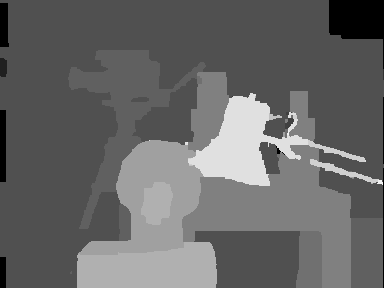
\includegraphics{pics/disparity.png}

\else

\lstinputlisting{python_fragments/findstereocorrespondence.py}

and this is the output left disparity image computed from the well-known
Tsukuba stereo pair and multiplied by -16 (because the values in the
left disparity images are usually negative):

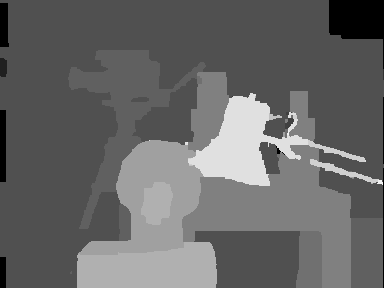
\includegraphics{pics/disparity.png}

\fi

\fi

\ifCpp
\cvCppFunc{getDefaultNewCameraMatrix}
Returns the default new camera matrix

\cvdefCpp{Mat getDefaultNewCameraMatrix(\par
                               const Mat\& cameraMatrix,\par
                               Size imgSize=Size(),\par
                               bool centerPrincipalPoint=false );}
\begin{description}
\cvarg{cameraMatrix}{The input camera matrix}
\cvarg{imageSize}{The camera view image size in pixels}
\cvarg{centerPrincipalPoint}{Indicates whether in the new camera matrix the principal point should be at the image center or not}
\end{description}

The function returns the camera matrix that is either an exact copy of the input \texttt{cameraMatrix} (when \texttt{centerPrinicipalPoint=false}), or the modified one (when \texttt{centerPrincipalPoint}=true).

In the latter case the new camera matrix will be:

\[\begin{bmatrix}
f_x && 0 && (\texttt{imgSize.width}-1)*0.5 \\
0 && f_y && (\texttt{imgSize.height}-1)*0.5 \\
0 && 0 && 1
\end{bmatrix},\]

where $f_x$ and $f_y$ are $(0,0)$ and $(1,1)$ elements of \texttt{cameraMatrix}, respectively.

By default, the undistortion functions in OpenCV (see \texttt{initUndistortRectifyMap}, \texttt{undistort}) do not move the principal point. However, when you work with stereo, it's important to move the principal points in both views to the same y-coordinate (which is required by most of stereo correspondence algorithms), and maybe to the same x-coordinate too. So you can form the new camera matrix for each view, where the principal points will be at the center.

\fi

\ifCPy
\cvCPyFunc{GetOptimalNewCameraMatrix}
\else
\cvCppFunc{getOptimalNewCameraMatrix}
\fi
Returns the new camera matrix based on the free scaling parameter

\cvdefC{void cvGetOptimalNewCameraMatrix(
    \par const CvMat* cameraMatrix, const CvMat* distCoeffs,
    \par CvSize imageSize, double alpha,
    \par CvMat* newCameraMatrix,
    \par CvSize newImageSize=cvSize(0,0),
    \par CvRect* validPixROI=0 );}
\cvdefPy{GetOptimalNewCameraMatrix(cameraMatrix, distCoeffs, imageSize, alpha, newCameraMatrix, newImageSize=(0,0), validPixROI=0) -> None}
\cvdefCpp{Mat getOptimalNewCameraMatrix(
    \par const Mat\& cameraMatrix, const Mat\& distCoeffs,
    \par Size imageSize, double alpha, Size newImageSize=Size(),
    \par Rect* validPixROI=0);}
    
\begin{description}
\cvarg{cameraMatrix}{The input camera matrix}
\cvarg{distCoeffs}{The input vector of distortion coefficients $(k_1, k_2, p_1, p_2[, k_3[, k_4, k_5, k_6]])$ of 4, 5 or 8 elements. If the vector is NULL/empty, the zero distortion coefficients are assumed.}
\cvarg{imageSize}{The original image size}
\cvarg{alpha}{The free scaling parameter between 0 (when all the pixels in the undistorted image will be valid) and 1 (when all the source image pixels will be retained in the undistorted image); see \cvCross{StereoRectify}{stereoRectify}}
\cvarg{newCameraMatrix}{The output new camera matrix.}
\cvarg{newImageSize}{The image size after rectification. By default it will be set to \texttt{imageSize}.}
\cvarg{validPixROI}{The optional output rectangle that will outline all-good-pixels region in the undistorted image. See \texttt{roi1, roi2} description in \cvCross{StereoRectify}{stereoRectify}}
\end{description}

The function computes \cvCpp{and returns} the optimal new camera matrix based on the free scaling parameter. By varying  this parameter the user may retrieve only sensible pixels \texttt{alpha=0}, keep all the original image pixels if there is valuable information in the corners \texttt{alpha=1}, or get something in between. When \texttt{alpha>0}, the undistortion result will likely have some black pixels corresponding to "virtual" pixels outside of the captured distorted image. The original camera matrix, distortion coefficients, the computed new camera matrix and the \texttt{newImageSize} should be passed to \cvCross{InitUndistortRectifyMap}{initUndistortRectifyMap} to produce the maps for \cvCross{Remap}{remap}.

\ifCPy
\cvCPyFunc{InitIntrinsicParams2D}
\else
\cvCppFunc{initCameraMatrix2D}
\fi

Finds the initial camera matrix from the 3D-2D point correspondences

\cvdefC{void cvInitIntrinsicParams2D(\par const CvMat* objectPoints,
                                     \par const CvMat* imagePoints,
                                     \par const CvMat* npoints, CvSize imageSize,
                                     \par CvMat* cameraMatrix,
                                     \par double aspectRatio=1.);}                                     
\cvdefPy{InitIntrinsicParams2D(objectPoints, imagePoints, npoints, imageSize, cameraMatrix, aspectRatio=1.) -> None}
\cvdefCpp{Mat initCameraMatrix2D( const vector<vector<Point3f> >\& objectPoints,\par
                        const vector<vector<Point2f> >\& imagePoints,\par
                        Size imageSize, double aspectRatio=1.);}
\begin{description}
\ifCPy
\cvarg{objectPoints}{The joint array of object points; see \cvCross{CalibrateCamera2}{calibrateCamera}}
\cvarg{imagePoints}{The joint array of object point projections; see \cvCross{CalibrateCamera2}{calibrateCamera}}
\cvarg{npoints}{The array of point counts; see \cvCross{CalibrateCamera2}{calibrateCamera}}
\fi    
\ifCpp
\cvarg{objectPoints}{The vector of vectors of the object points. See \cvCppCross{calibrateCamera}}
\cvarg{imagePoints}{The vector of vectors of the corresponding image points. See \cvCppCross{calibrateCamera}}
\fi
\cvarg{imageSize}{The image size in pixels; used to initialize the principal point}
\cvCPy{\cvarg{cameraMatrix}{The output camera matrix $\vecthreethree{f_x}{0}{c_x}{0}{f_y}{c_y}{0}{0}{1}$}}
\cvarg{aspectRatio}{If it is zero or negative, both $f_x$ and $f_y$ are estimated independently. Otherwise $f_x = f_y * \texttt{aspectRatio}$}
\end{description}

The function estimates and returns the initial camera matrix for camera calibration process.
Currently, the function only supports planar calibration patterns, i.e. patterns where each object point has z-coordinate =0.

\ifCPy
\cvCPyFunc{InitUndistortMap}
Computes an undistortion map.

\cvdefC{void cvInitUndistortMap( \par const CvMat* cameraMatrix,\par const CvMat* distCoeffs,\par CvArr* map1,\par CvArr* map2 );}
\cvdefPy{InitUndistortMap(cameraMatrix,distCoeffs,map1,map2)-> None}

\begin{description}
\cvarg{cameraMatrix}{The input camera matrix $A = \vecthreethree{fx}{0}{cx}{0}{fy}{cy}{0}{0}{1} $}
\cvarg{distCoeffs}{The input vector of distortion coefficients $(k_1, k_2, p_1, p_2[, k_3[, k_4, k_5, k_6]])$ of 4, 5 or 8 elements. If the vector is NULL/empty, the zero distortion coefficients are assumed.}
\cvarg{map1}{The first output map \cvCPy{of type \texttt{CV\_32FC1} or \texttt{CV\_16SC2} - the second variant is more efficient}}
\cvarg{map2}{The second output map \cvCPy{of type \texttt{CV\_32FC1} or \texttt{CV\_16UC1} - the second variant is more efficient}}
\end{description}

The function is a simplified variant of \cvCross{InitUndistortRectifyMap}{initUndistortRectifyMap} where the rectification transformation \texttt{R} is identity matrix and \texttt{newCameraMatrix=cameraMatrix}.

\fi

\ifCPy
\cvCPyFunc{InitUndistortRectifyMap}
\else
\cvCppFunc{initUndistortRectifyMap}
\fi
Computes the undistortion and rectification transformation map.

\cvdefC{void cvInitUndistortRectifyMap( \par const CvMat* cameraMatrix,
                                \par const CvMat* distCoeffs,
                                \par const CvMat* R,
                                \par const CvMat* newCameraMatrix,
                                \par CvArr* map1, \par CvArr* map2 );}
\cvdefPy{InitUndistortRectifyMap(cameraMatrix,distCoeffs,R,newCameraMatrix,map1,map2)-> None}
\cvdefCpp{void initUndistortRectifyMap( const Mat\& cameraMatrix,\par
                           const Mat\& distCoeffs, const Mat\& R,\par
                           const Mat\& newCameraMatrix,\par
                           Size size, int m1type,\par
                           Mat\& map1, Mat\& map2 );}
\begin{description}
\cvarg{cameraMatrix}{The input camera matrix $A=\vecthreethree{f_x}{0}{c_x}{0}{f_y}{c_y}{0}{0}{1}$}
\cvarg{distCoeffs}{The input vector of distortion coefficients $(k_1, k_2, p_1, p_2[, k_3[, k_4, k_5, k_6]])$ of 4, 5 or 8 elements. If the vector is NULL/empty, the zero distortion coefficients are assumed.}
\cvarg{R}{The optional rectification transformation in object space (3x3 matrix). \texttt{R1} or \texttt{R2}, computed by \cvCross{StereoRectify}{stereoRectify} can be passed here. If the matrix is \cvCPy{NULL}\cvCpp{empty}, the identity transformation is assumed}
\cvarg{newCameraMatrix}{The new camera matrix $A'=\vecthreethree{f_x'}{0}{c_x'}{0}{f_y'}{c_y'}{0}{0}{1}$}
\cvCpp{\cvarg{size}{The undistorted image size}
\cvarg{m1type}{The type of the first output map, can be \texttt{CV\_32FC1} or \texttt{CV\_16SC2}. See \cvCppCross{convertMaps}}}
\cvarg{map1}{The first output map \cvCPy{of type \texttt{CV\_32FC1} or \texttt{CV\_16SC2} - the second variant is more efficient}}
\cvarg{map2}{The second output map \cvCPy{of type \texttt{CV\_32FC1} or \texttt{CV\_16UC1} - the second variant is more efficient}}
\end{description}

The function computes the joint undistortion+rectification transformation and represents the result in the form of maps for \cvCross{Remap}{remap}. The undistorted image will look like the original, as if it was captured with a camera with camera matrix \texttt{=newCameraMatrix} and zero distortion. In the case of monocular camera \texttt{newCameraMatrix} is usually equal to \texttt{cameraMatrix}, or it can be computed by \cvCross{GetOptimalNewCameraMatrix}{getOptimalNewCameraMatrix} for a better control over scaling. In the case of stereo camera \texttt{newCameraMatrix} is normally set to \texttt{P1} or \texttt{P2} computed by \cvCross{StereoRectify}{stereoRectify}.

Also, this new camera will be oriented differently in the coordinate space, according to \texttt{R}. That, for example, helps to align two heads of a stereo camera so that the epipolar lines on both images become horizontal and have the same y- coordinate (in the case of horizontally aligned stereo camera).

The function actually builds the maps for the inverse mapping algorithm that is used by \cvCross{Remap}{remap}. That is, for each pixel $(u, v)$ in the destination (corrected and rectified) image the function computes the corresponding coordinates in the source image (i.e. in the original image from camera). The process is the following:

\[
\begin{array}{l}
x \leftarrow (u - {c'}_x)/{f'}_x \\
y \leftarrow (v - {c'}_y)/{f'}_y \\
{[X\,Y\,W]}^T \leftarrow R^{-1}*[x\,y\,1]^T \\
x' \leftarrow X/W \\
y' \leftarrow Y/W \\
x" \leftarrow x' (1 + k_1 r^2 + k_2 r^4 + k_3 r^6) + 2p_1 x' y' + p_2(r^2 + 2 x'^2) \\
y" \leftarrow y' (1 + k_1 r^2 + k_2 r^4 + k_3 r^6) + p_1 (r^2 + 2 y'^2) + 2 p_2 x' y' \\
map_x(u,v) \leftarrow x" f_x + c_x \\
map_y(u,v) \leftarrow y" f_y + c_y
\end{array}
\]
where $(k_1, k_2, p_1, p_2[, k_3])$ are the distortion coefficients. 
 
In the case of a stereo camera this function is called twice, once for each camera head, after \cvCross{StereoRectify}{stereoRectify}, which in its turn is called after \cvCross{StereoCalibrate}{stereoCalibrate}. But if the stereo camera was not calibrated, it is still possible to compute the rectification transformations directly from the fundamental matrix using \cvCross{StereoRectifyUncalibrated}{stereoRectifyUncalibrated}. For each camera the function computes homography \texttt{H} as the rectification transformation in pixel domain, not a rotation matrix \texttt{R} in 3D space. The \texttt{R} can be computed from \texttt{H} as 

\[ \texttt{R} = \texttt{cameraMatrix}^{-1} \cdot \texttt{H} \cdot \texttt{cameraMatrix} \]

where the \texttt{cameraMatrix} can be chosen arbitrarily.

\ifCpp

\cvCppFunc{matMulDeriv}
Computes partial derivatives of the matrix product w.r.t each multiplied matrix

\cvdefCpp{void matMulDeriv( const Mat\& A, const Mat\& B, Mat\& dABdA, Mat\& dABdB );}
\begin{description}
\cvarg{A}{The first multiplied matrix}
\cvarg{B}{The second multiplied matrix}
\cvarg{dABdA}{The first output derivative matrix \texttt{d(A*B)/dA} of size $\texttt{A.rows*B.cols} \times {A.rows*A.cols}$}
\cvarg{dABdA}{The second output derivative matrix \texttt{d(A*B)/dB} of size $\texttt{A.rows*B.cols} \times {B.rows*B.cols}$}
\end{description}

The function computes the partial derivatives of the elements of the matrix product $A*B$ w.r.t. the elements of each of the two input matrices. The function is used to compute Jacobian matrices in \cvCppCross{stereoCalibrate}, but can also be used in any other similar optimization function.

\fi

\ifCPy

\cvCPyFunc{POSIT}
Implements the POSIT algorithm.

\cvdefC{
void cvPOSIT( \par CvPOSITObject* posit\_object,\par CvPoint2D32f* imagePoints,\par double focal\_length,\par CvTermCriteria criteria,\par CvMatr32f rotationMatrix,\par CvVect32f translation\_vector );
}
\cvdefPy{POSIT(posit\_object,imagePoints,focal\_length,criteria)-> (rotationMatrix,translation\_vector)}

\begin{description}
\cvarg{posit\_object}{Pointer to the object structure}
\cvarg{imagePoints}{Pointer to the object points projections on the 2D image plane}
\cvarg{focal\_length}{Focal length of the camera used}
\cvarg{criteria}{Termination criteria of the iterative POSIT algorithm}
\cvarg{rotationMatrix}{Matrix of rotations}
\cvarg{translation\_vector}{Translation vector}
\end{description}

The function implements the POSIT algorithm. Image coordinates are given in a camera-related coordinate system. The focal length may be retrieved using the camera calibration functions. At every iteration of the algorithm a new perspective projection of the estimated pose is computed.

Difference norm between two projections is the maximal distance between corresponding points. The parameter \texttt{criteria.epsilon} serves to stop the algorithm if the difference is small.

\fi

\ifCPy
\cvCPyFunc{ProjectPoints2}
\else
\cvCppFunc{projectPoints}
\fi
Project 3D points on to an image plane.

\cvdefC{void cvProjectPoints2( \par const CvMat* objectPoints,\par const CvMat* rvec,\par const CvMat* tvec,\par const CvMat* cameraMatrix,\par const CvMat* distCoeffs,\par CvMat* imagePoints,\par CvMat* dpdrot=NULL,\par CvMat* dpdt=NULL,\par CvMat* dpdf=NULL,\par CvMat* dpdc=NULL,\par CvMat* dpddist=NULL );}

\cvdefPy{ProjectPoints2(objectPoints,rvec,tvec,cameraMatrix,distCoeffs, imagePoints,dpdrot=NULL,dpdt=NULL,dpdf=NULL,dpdc=NULL,dpddist=NULL)-> None}


\cvdefCpp{void projectPoints( const Mat\& objectPoints,\par
                    const Mat\& rvec, const Mat\& tvec,\par
                    const Mat\& cameraMatrix,\par
                    const Mat\& distCoeffs,\par
                    vector<Point2f>\& imagePoints );\newline
void projectPoints( const Mat\& objectPoints,\par
                    const Mat\& rvec, const Mat\& tvec,\par
                    const Mat\& cameraMatrix,\par
                    const Mat\& distCoeffs,\par
                    vector<Point2f>\& imagePoints,\par
                    Mat\& dpdrot, Mat\& dpdt, Mat\& dpdf,\par
                    Mat\& dpdc, Mat\& dpddist,\par
                    double aspectRatio=0 );}

\begin{description}
\cvarg{objectPoints}{The array of object points, 3xN or Nx3 1-channel or 1xN or Nx1 3-channel \cvCpp{(or \texttt{vector<Point3f>})}, where N is the number of points in the view}
\cvarg{rvec}{The rotation vector, see \cvCross{Rodrigues2}{Rodrigues}}
\cvarg{tvec}{The translation vector}
\cvarg{cameraMatrix}{The camera matrix $A = \vecthreethree{f_x}{0}{c_x}{0}{f_y}{c_y}{0}{0}{_1} $}
\cvarg{distCoeffs}{The input vector of distortion coefficients $(k_1, k_2, p_1, p_2[, k_3[, k_4, k_5, k_6]])$ of 4, 5 or 8 elements. If the vector is NULL/empty, the zero distortion coefficients are assumed.}
\cvarg{imagePoints}{The output array of image points, 2xN or Nx2 1-channel or 1xN or Nx1 2-channel \cvCpp{(or \texttt{vector<Point2f>})}}
\cvarg{dpdrot}{Optional 2Nx3 matrix of derivatives of image points with respect to components of the rotation vector}
\cvarg{dpdt}{Optional 2Nx3 matrix of derivatives of image points with respect to components of the translation vector}
\cvarg{dpdf}{Optional 2Nx2 matrix of derivatives of image points with respect to $f_x$ and $f_y$}
\cvarg{dpdc}{Optional 2Nx2 matrix of derivatives of image points with respect to $c_x$ and $c_y$}
\cvarg{dpddist}{Optional 2Nx4 matrix of derivatives of image points with respect to distortion coefficients}
\end{description}

The function computes projections of 3D
points to the image plane given intrinsic and extrinsic camera
parameters. Optionally, the function computes jacobians - matrices
of partial derivatives of image points coordinates (as functions of all the
input parameters) with respect to the particular parameters, intrinsic and/or
extrinsic. The jacobians are used during the global optimization
in \cvCross{CalibrateCamera2}{calibrateCamera},
\cvCross{FindExtrinsicCameraParams2}{solvePnP} and \cvCross{StereoCalibrate}{stereoCalibrate}. The
function itself can also used to compute re-projection error given the
current intrinsic and extrinsic parameters.

Note, that by setting \texttt{rvec=tvec=(0,0,0)}, or by setting \texttt{cameraMatrix} to 3x3 identity matrix, or by passing zero distortion coefficients, you can get various useful partial cases of the function, i.e. you can compute the distorted coordinates for a sparse set of points, or apply a perspective transformation (and also compute the derivatives) in the ideal zero-distortion setup etc.


\ifCPy
\cvCPyFunc{ReprojectImageTo3D}
\else
\cvCppFunc{reprojectImageTo3D}
\fi
Reprojects disparity image to 3D space.

\cvdefC{void cvReprojectImageTo3D( const CvArr* disparity,\par
                                   CvArr* \_3dImage, const CvMat* Q,\par
                                   int handleMissingValues=0);}

\cvdefPy{ReprojectImageTo3D(disparity, \_3dImage, Q, handleMissingValues=0) -> None}

\cvdefCpp{void reprojectImageTo3D( const Mat\& disparity,\par
                         Mat\& \_3dImage, const Mat\& Q,\par
                         bool handleMissingValues=false );}
\begin{description}
\cvarg{disparity}{The input single-channel 16-bit signed or 32-bit floating-point disparity image}
\cvarg{\_3dImage}{The output 3-channel floating-point image of the same size as \texttt{disparity}.
 Each element of \texttt{\_3dImage(x,y)} will contain the 3D coordinates of the point \texttt{(x,y)}, computed from the disparity map.}
\cvarg{Q}{The $4 \times 4$ perspective transformation matrix that can be obtained with \cvCross{StereoRectify}{stereoRectify}}
\cvarg{handleMissingValues}{If true, when the pixels with the minimal disparity (that corresponds to the outliers; see \cvCross{FindStereoCorrespondenceBM}{StereoBM}) will be transformed to 3D points with some very large Z value (currently set to 10000)}
\end{description}
 
The function transforms 1-channel disparity map to 3-channel image representing a 3D surface. That is, for each pixel \texttt{(x,y)} and the corresponding disparity \texttt{d=disparity(x,y)} it computes: 

\[\begin{array}{l}
[X\; Y\; Z\; W]^T = \texttt{Q}*[x\; y\; \texttt{disparity}(x,y)\; 1]^T \\
\texttt{\_3dImage}(x,y) = (X/W,\; Y/W,\; Z/W)
\end{array}\]

The matrix \texttt{Q} can be arbitrary $4 \times 4$ matrix, e.g. the one computed by \cvCross{StereoRectify}{stereoRectify}. To reproject a sparse set of points {(x,y,d),...} to 3D space, use \cvCross{PerspectiveTransform}{perspectiveTransform}.

\ifCPy
\cvCPyFunc{RQDecomp3x3}
\else
\cvCppFunc{RQDecomp3x3}
\fi
Computes the 'RQ' decomposition of 3x3 matrices.

\cvdefC{
void cvRQDecomp3x3( \par const CvMat *M,\par CvMat *R,\par CvMat *Q,\par CvMat *Qx=NULL,\par CvMat *Qy=NULL,\par CvMat *Qz=NULL,\par CvPoint3D64f *eulerAngles=NULL);
}
\cvdefPy{RQDecomp3x3(M, R, Q, Qx = None, Qy = None, Qz = None) -> eulerAngles}
\cvdefCpp{void RQDecomp3x3( const Mat\& M, Mat\& R, Mat\& Q );\newline
Vec3d RQDecomp3x3( const Mat\& M, Mat\& R, Mat\& Q,\par
                   Mat\& Qx, Mat\& Qy, Mat\& Qz );}

\begin{description}
\cvarg{M}{The 3x3 input matrix}
\cvarg{R}{The output 3x3 upper-triangular matrix}
\cvarg{Q}{The output 3x3 orthogonal matrix}
\cvarg{Qx}{Optional 3x3 rotation matrix around x-axis}
\cvarg{Qy}{Optional 3x3 rotation matrix around y-axis}
\cvarg{Qz}{Optional 3x3 rotation matrix around z-axis}
\cvCPy{\cvarg{eulerAngles}{Optional three Euler angles of rotation}}
\end{description}

The function computes a RQ decomposition using the given rotations. This function is used in \cvCross{DecomposeProjectionMatrix}{decomposeProjectionMatrix} to decompose the left 3x3 submatrix of a projection matrix into a camera and a rotation matrix.

It optionally returns three rotation matrices, one for each axis, and the three Euler angles \cvCpp{(as the return value)} that could be used in OpenGL.

\ifC

\cvCPyFunc{ReleasePOSITObject}
Deallocates a 3D object structure.

\cvdefC{
void cvReleasePOSITObject( \par CvPOSITObject** posit\_object );
}

\begin{description}
\cvarg{posit\_object}{Double pointer to \texttt{CvPOSIT} structure}
\end{description}

The function releases memory previously allocated by the function \cvCPyCross{CreatePOSITObject}.

\fi

\ifC

\cvCPyFunc{ReleaseStereoBMState}
Releases block matching stereo correspondence structure.

\cvdefC{void cvReleaseStereoBMState( CvStereoBMState** state );}
\cvdefPy{ReleaseStereoBMState(state)-> None}

\begin{description}
\cvarg{state}{Double pointer to the released structure.}
\end{description}

The function releases the stereo correspondence structure and all the associated internal buffers. 

\cvCPyFunc{ReleaseStereoGCState}
Releases the state structure of the graph cut-based stereo correspondence algorithm.

\cvdefC{void cvReleaseStereoGCState( CvStereoGCState** state );}
\cvdefPy{ReleaseStereoGCState(state)-> None}

\begin{description}
\cvarg{state}{Double pointer to the released structure.}
\end{description}

The function releases the stereo correspondence structure and all the associated internal buffers. 

\fi

\ifCPy
\cvCPyFunc{Rodrigues2}
\else
\cvCppFunc{Rodrigues}
\fi
Converts a rotation matrix to a rotation vector or vice versa.

\cvdefC{int cvRodrigues2( \par const CvMat* src,\par CvMat* dst,\par CvMat* jacobian=0 );}
\cvdefPy{Rodrigues2(src,dst,jacobian=0)-> None}

\cvdefCpp{void Rodrigues(const Mat\& src, Mat\& dst);\newline
void Rodrigues(const Mat\& src, Mat\& dst, Mat\& jacobian);}

\begin{description}
\cvarg{src}{The input rotation vector (3x1 or 1x3) or rotation matrix (3x3)}
\cvarg{dst}{The output rotation matrix (3x3) or rotation vector (3x1 or 1x3), respectively}
\cvarg{jacobian}{Optional output Jacobian matrix, 3x9 or 9x3 - partial derivatives of the output array components with respect to the input array components}
\end{description}

\[
\begin{array}{l}
\theta \leftarrow norm(r)\\
r \leftarrow r/\theta\\
R = \cos{\theta} I + (1-\cos{\theta}) r r^T + \sin{\theta}
\vecthreethree
{0}{-r_z}{r_y}
{r_z}{0}{-r_x}
{-r_y}{r_x}{0}
\end{array}
\]

Inverse transformation can also be done easily, since

\[
\sin(\theta)
\vecthreethree
{0}{-r_z}{r_y}
{r_z}{0}{-r_x}
{-r_y}{r_x}{0}
=
\frac{R - R^T}{2}
\]

A rotation vector is a convenient and most-compact representation of a rotation matrix
(since any rotation matrix has just 3 degrees of freedom). The representation is
used in the global 3D geometry optimization procedures like \cvCross{CalibrateCamera2}{calibrateCamera},
\cvCross{StereoCalibrate}{stereoCalibrate} or \cvCross{FindExtrinsicCameraParams2}{solvePnP}.


\ifCpp

\cvclass{StereoBM}
The class for computing stereo correspondence using block matching algorithm.

\begin{lstlisting}
// Block matching stereo correspondence algorithm\par
class StereoBM
{
    enum { NORMALIZED_RESPONSE = CV_STEREO_BM_NORMALIZED_RESPONSE,
        BASIC_PRESET=CV_STEREO_BM_BASIC,
        FISH_EYE_PRESET=CV_STEREO_BM_FISH_EYE,
        NARROW_PRESET=CV_STEREO_BM_NARROW };

    StereoBM();
    // the preset is one of ..._PRESET above.
    // ndisparities is the size of disparity range,
    // in which the optimal disparity at each pixel is searched for.
    // SADWindowSize is the size of averaging window used to match pixel blocks
    //    (larger values mean better robustness to noise, but yield blurry disparity maps)
    StereoBM(int preset, int ndisparities=0, int SADWindowSize=21);
    // separate initialization function
    void init(int preset, int ndisparities=0, int SADWindowSize=21);
    // computes the disparity for the two rectified 8-bit single-channel images.
    // the disparity will be 16-bit signed (fixed-point) or 32-bit floating-point image of the same size as left.
    void operator()( const Mat& left, const Mat& right, Mat& disparity, int disptype=CV_16S );

    Ptr<CvStereoBMState> state;
};
\end{lstlisting}

The class is a C++ wrapper for \hyperref[CvStereoBMState]{cvStereoBMState} and the associated functions. In particular, \texttt{StereoBM::operator ()} is the wrapper for \cvCPyCross{FindStereoCorrespondceBM}. See the respective descriptions.


\cvclass{StereoSGBM}
The class for computing stereo correspondence using semi-global block matching algorithm.

\begin{lstlisting}
class StereoSGBM
{
    StereoSGBM();
    StereoSGBM(int minDisparity, int numDisparities, int SADWindowSize,
               int P1=0, int P2=0, int disp12MaxDiff=0,
               int preFilterCap=0, int uniquenessRatio=0,
               int speckleWindowSize=0, int speckleRange=0,
               bool fullDP=false);
    virtual ~StereoSGBM();
    
    virtual void operator()(const Mat& left, const Mat& right, Mat& disp);
    
    int minDisparity;
    int numberOfDisparities;
    int SADWindowSize;
    int preFilterCap;
    int uniquenessRatio;
    int P1, P2;
    int speckleWindowSize;
    int speckleRange;
    int disp12MaxDiff;
    bool fullDP;
    
    ...
};
\end{lstlisting}

The class implements modified H. Hirschmuller algorithm \cite{HH08}. The main differences between the implemented algorithm and the original one are:

\begin{itemize}
    \item by default the algorithm is single-pass, i.e. instead of 8 directions we only consider 5. Set \texttt{fullDP=true} to run the full variant of the algorithm (which could consume \emph{a lot} of memory)
    \item the algorithm matches blocks, not individual pixels (though, by setting \texttt{SADWindowSize=1} the blocks are reduced to single pixels)
    \item mutual information cost function is not implemented. Instead, we use a simpler Birchfield-Tomasi sub-pixel metric from \cite{BT96}, though the color images are supported as well.
    \item we include some pre- and post- processing steps from K. Konolige algorithm \cvCPyCross{FindStereoCorrespondceBM}, such as pre-filtering (\texttt{CV\_STEREO\_BM\_XSOBEL} type) and post-filtering (uniqueness check, quadratic interpolation and speckle filtering)
\end{itemize}

\cvCppFunc{StereoSGBM::StereoSGBM}
StereoSGBM constructors

\cvdefCpp{
StereoSGBM::StereoSGBM();\newline
StereoSGBM::StereoSGBM(
            \par int minDisparity, int numDisparities, int SADWindowSize,
           \par int P1=0, int P2=0, int disp12MaxDiff=0,
           \par int preFilterCap=0, int uniquenessRatio=0,
           \par int speckleWindowSize=0, int speckleRange=0,
           \par bool fullDP=false);
}
\begin{description}
\cvarg{minDisparity}{The minimum possible disparity value. Normally it is 0, but sometimes rectification algorithms can shift images, so this parameter needs to be adjusted accordingly}
\cvarg{numDisparities}{This is maximum disparity minus minimum disparity. Always greater than 0. In the current implementation this parameter must be divisible by 16.}
\cvarg{SADWindowSize}{The matched block size. Must be an odd number \texttt{>=1}. Normally, it should be somewhere in \texttt{3..11} range}.
\cvarg{P1, P2}{Parameters that control disparity smoothness. The larger the values, the smoother the disparity. \texttt{P1} is the penalty on the disparity change by plus or minus 1 between neighbor pixels. \texttt{P2} is the penalty on the disparity change by more than 1 between neighbor pixels. The algorithm requires \texttt{P2 > P1}. See \texttt{stereo\_match.cpp} sample where some reasonably good \texttt{P1} and \texttt{P2} values are shown (like \texttt{8*number\_of\_image\_channels*SADWindowSize*SADWindowSize} and \texttt{32*number\_of\_image\_channels*SADWindowSize*SADWindowSize}, respectively).}
\cvarg{disp12MaxDiff}{Maximum allowed difference (in integer pixel units) in the left-right disparity check. Set it to non-positive value to disable the check.}
\cvarg{preFilterCap}{Truncation value for the prefiltered image pixels. The algorithm first computes x-derivative at each pixel and clips its value by \texttt{[-preFilterCap, preFilterCap]} interval. The result values are passed to the Birchfield-Tomasi pixel cost function.}
\cvarg{uniquenessRatio}{The margin in percents by which the best (minimum) computed cost function value should "win" the second best value to consider the found match correct. Normally, some value within 5-15 range is good enough}
\cvarg{speckleWindowSize}{Maximum size of smooth disparity regions to consider them noise speckles and invdalidate. Set it to 0 to disable speckle filtering. Otherwise, set it somewhere in 50-200 range.}
\cvarg{speckleRange}{Maximum disparity variation within each connected component. If you do speckle filtering, set it to some positive value, multiple of 16. Normally, 16 or 32 is good enough.}
\cvarg{fullDP}{Set it to \texttt{true} to run full-scale 2-pass dynamic programming algorithm. It will consume O(W*H*numDisparities) bytes, which is large for 640x480 stereo and huge for HD-size pictures. By default this is \texttt{false}}
\end{description}

The first constructor initializes \texttt{StereoSGBM} with all the default parameters (so actually one will only have to set \texttt{StereoSGBM::numberOfDisparities} at minimum). The second constructor allows you to set each parameter to a custom value.

\cvCppFunc{StereoSGBM::operator ()}
Computes disparity using SGBM algorithm for a rectified stereo pair

\cvdefCpp{
void SGBM::operator()(const Mat\& left, const Mat\& right, Mat\& disp);
}
\begin{description}
\cvarg{left}{The left image, 8-bit single-channel or 3-channel.}
\cvarg{right}{The right image of the same size and the same type as the left one.}
\cvarg{disp}{The output disparity map. It will be 16-bit signed single-channel image of the same size as the input images. It will contain scaled by 16 disparity values, so that to get the floating-point disparity map, you will need to divide each \texttt{disp} element by 16.}
\end{description}

The method executes SGBM algorithm on a rectified stereo pair. See \texttt{stereo\_match.cpp} OpenCV sample on how to prepare the images and call the method. Note that the method is not constant, thus you should not use the same \texttt{StereoSGBM} instance from within different threads simultaneously.

\fi

\ifCPy
\cvCPyFunc{StereoCalibrate}
\else
\cvCppFunc{stereoCalibrate}
\fi
Calibrates stereo camera.

\cvdefC{double cvStereoCalibrate( \par const CvMat* objectPoints, \par const CvMat* imagePoints1,
                        \par const CvMat* imagePoints2, \par const CvMat* pointCounts,
                        \par CvMat* cameraMatrix1, \par CvMat* distCoeffs1,
                        \par CvMat* cameraMatrix2, \par CvMat* distCoeffs2,
                       \par CvSize imageSize, \par CvMat* R, \par CvMat* T,
                        \par CvMat* E=0, \par CvMat* F=0,
                        \par CvTermCriteria term\_crit=cvTermCriteria(
                               \par CV\_TERMCRIT\_ITER+CV\_TERMCRIT\_EPS,30,1e-6),
                        \par int flags=CV\_CALIB\_FIX\_INTRINSIC );}

\cvdefPy{StereoCalibrate( objectPoints, imagePoints1, imagePoints2, pointCounts, cameraMatrix1, distCoeffs1, cameraMatrix2, distCoeffs2, imageSize, R, T, E=NULL, F=NULL, term\_crit=(CV\_TERMCRIT\_ITER+CV\_TERMCRIT\_EPS,30,1e-6), flags=CV\_CALIB\_FIX\_INTRINSIC)-> None}

\cvdefCpp{double stereoCalibrate( const vector<vector<Point3f> >\& objectPoints,\par
                      const vector<vector<Point2f> >\& imagePoints1,\par
                      const vector<vector<Point2f> >\& imagePoints2,\par
                      Mat\& cameraMatrix1, Mat\& distCoeffs1,\par
                      Mat\& cameraMatrix2, Mat\& distCoeffs2,\par
                      Size imageSize, Mat\& R, Mat\& T,\par
                      Mat\& E, Mat\& F,\par
                      TermCriteria term\_crit = TermCriteria(TermCriteria::COUNT+\par
                         TermCriteria::EPS, 30, 1e-6),\par
                      int flags=CALIB\_FIX\_INTRINSIC );}

\begin{description}
\ifCPy
    \cvarg{objectPoints}{The joint matrix of object points - calibration pattern features in the model coordinate space. It is floating-point 3xN or Nx3 1-channel, or 1xN or Nx1 3-channel array, where N is the total number of points in all views.}
    \cvarg{imagePoints1}{The joint matrix of object points projections in the first camera views. It is floating-point 2xN or Nx2 1-channel, or 1xN or Nx1 2-channel array, where N is the total number of points in all views}
    \cvarg{imagePoints2}{The joint matrix of object points projections in the second camera views. It is floating-point 2xN or Nx2 1-channel, or 1xN or Nx1 2-channel array, where N is the total number of points in all views}
    \cvarg{pointCounts}{Integer 1xM or Mx1 vector (where M is the number of calibration pattern views) containing the number of points in each particular view. The sum of vector elements must match the size of \texttt{objectPoints} and \texttt{imagePoints*} (=N).}
\fi
\ifCpp
    \cvarg{objectPoints}{The vector of vectors of points on the calibration pattern in its coordinate system, one vector per view. If the same calibration pattern is shown in each view and it's fully visible then all the vectors will be the same, although it is possible to use partially occluded patterns, or even different patterns in different views - then the vectors will be different. The points are 3D, but since they are in the pattern coordinate system, then if the rig is planar, it may have sense to put the model to the XY coordinate plane, so that Z-coordinate of each input object point is 0}
    \cvarg{imagePoints1}{The vector of vectors of the object point projections on the calibration pattern views from the 1st camera, one vector per a view. The projections must be in the same order as the corresponding object points.}
    \cvarg{imagePoints2}{The vector of vectors of the object point projections on the calibration pattern views from the 2nd camera, one vector per a view. The projections must be in the same order as the corresponding object points.}
\fi
    \cvarg{cameraMatrix1}{The input/output first camera matrix: $ \vecthreethree{f_x^{(j)}}{0}{c_x^{(j)}}{0}{f_y^{(j)}}{c_y^{(j)}}{0}{0}{1}$, $j = 0,\, 1$. If any of \texttt{CV\_CALIB\_USE\_INTRINSIC\_GUESS}, \newline \texttt{CV\_CALIB\_FIX\_ASPECT\_RATIO}, \texttt{CV\_CALIB\_FIX\_INTRINSIC} or \texttt{CV\_CALIB\_FIX\_FOCAL\_LENGTH} are specified, some or all of the matrices' components must be initialized; see the flags description}
    \cvarg{distCoeffs}{The input/output vector of distortion coefficients $(k_1, k_2, p_1, p_2[, k_3[, k_4, k_5, k_6]])$ of 4, 5 or 8 elements. \cvCpp{On output vector length depends on the flags.}}
    \cvarg{cameraMatrix2}{The input/output second camera matrix, as cameraMatrix1.}
    \cvarg{distCoeffs2}{The input/output lens distortion coefficients for the second camera, as \texttt{distCoeffs1}.}
\cvarg{imageSize}{Size of the image, used only to initialize intrinsic camera matrix.} 
\cvarg{R}{The output rotation matrix between the 1st and the 2nd cameras' coordinate systems.}
\cvarg{T}{The output translation vector between the cameras' coordinate systems.}
\cvarg{E}{The \cvCPy{optional} output essential matrix.}
\cvarg{F}{The \cvCPy{optional} output fundamental matrix.}
\cvarg{term\_crit}{The termination criteria for the iterative optimization algorithm.}
\cvarg{flags}{Different flags, may be 0 or combination of the following values:
\begin{description}
\cvarg{CV\_CALIB\_FIX\_INTRINSIC}{If it is set, \texttt{cameraMatrix?}, as well as \texttt{distCoeffs?} are fixed, so that only \texttt{R, T, E} and \texttt{F} are estimated.}
\cvarg{CV\_CALIB\_USE\_INTRINSIC\_GUESS}{The flag allows the function to optimize some or all of the intrinsic parameters, depending on the other flags, but the initial values are provided by the user.}
\cvarg{CV\_CALIB\_FIX\_PRINCIPAL\_POINT}{The principal points are fixed during the optimization.}
\cvarg{CV\_CALIB\_FIX\_FOCAL\_LENGTH}{$f^{(j)}_x$ and $f^{(j)}_y$ are fixed.}
\cvarg{CV\_CALIB\_FIX\_ASPECT\_RATIO}{$f^{(j)}_y$ is optimized, but the ratio $f^{(j)}_x/f^{(j)}_y$ is fixed.}
\cvarg{CV\_CALIB\_SAME\_FOCAL\_LENGTH}{Enforces $f^{(0)}_x=f^{(1)}_x$ and $f^{(0)}_y=f^{(1)}_y$} \cvarg{CV\_CALIB\_ZERO\_TANGENT\_DIST}{Tangential distortion coefficients for each camera are set to zeros and fixed there.}
\cvarg{CV\_CALIB\_FIX\_K1,...,CV\_CALIB\_FIX\_K6}{Do not change the corresponding radial distortion coefficient during the optimization. If \texttt{CV\_CALIB\_USE\_INTRINSIC\_GUESS} is set, the coefficient from the supplied \texttt{distCoeffs} matrix is used, otherwise it is set to 0.}
\cvarg{CV\_CALIB\_RATIONAL\_MODEL}{Enable coefficients k4, k5 and k6. To provide the backward compatibility, this extra flag should be explicitly specified to make the calibration function use the rational model and return 8 coefficients. If the flag is not set, the function will compute \cvCpp{and return} only 5 distortion coefficients.}
\end{description}}
\end{description}

The function estimates transformation between the 2 cameras making a stereo pair. If we have a stereo camera, where the relative position and orientation of the 2 cameras is fixed, and if we computed poses of an object relative to the fist camera and to the second camera, (R1, T1) and (R2, T2), respectively (that can be done with \cvCross{FindExtrinsicCameraParams2}{solvePnP}), obviously, those poses will relate to each other, i.e. given ($R_1$, $T_1$) it should be possible to compute ($R_2$, $T_2$) - we only need to know the position and orientation of the 2nd camera relative to the 1st camera. That's what the described function does. It computes ($R$, $T$) such that:

\[
R_2=R*R_1
T_2=R*T_1 + T,
\]

Optionally, it computes the essential matrix E:

\[
E=
\vecthreethree
{0}{-T_2}{T_1}
{T_2}{0}{-T_0}
{-T_1}{T_0}{0}
*R
\]

where $T_i$ are components of the translation vector $T$: $T=[T_0, T_1, T_2]^T$. And also the function can compute the fundamental matrix F:

\[F = cameraMatrix2^{-T} E cameraMatrix1^{-1}\]

Besides the stereo-related information, the function can also perform full calibration of each of the 2 cameras. However, because of the high dimensionality of the parameter space and noise in the input data the function can diverge from the correct solution. Thus, if intrinsic parameters can be estimated with high accuracy for each of the cameras individually (e.g. using \cvCross{CalibrateCamera2}{calibrateCamera}), it is recommended to do so and then pass \texttt{CV\_CALIB\_FIX\_INTRINSIC} flag to the function along with the computed intrinsic parameters. Otherwise, if all the parameters are estimated at once, it makes sense to restrict some parameters, e.g. pass \texttt{CV\_CALIB\_SAME\_FOCAL\_LENGTH} and \texttt{CV\_CALIB\_ZERO\_TANGENT\_DIST} flags, which are usually reasonable assumptions.

Similarly to \cvCross{CalibrateCamera2}{calibrateCamera}, the function minimizes the total re-projection error for all the points in all the available views from both cameras.
\ifPy
\else
The function returns the final value of the re-projection error.
\fi

\ifCPy
\cvCPyFunc{StereoRectify}
\else
\cvCppFunc{stereoRectify}
\fi
Computes rectification transforms for each head of a calibrated stereo camera.

\cvdefC{void cvStereoRectify( \par const CvMat* cameraMatrix1, const CvMat* cameraMatrix2,
                      \par const CvMat* distCoeffs1, const CvMat* distCoeffs2,
                      \par CvSize imageSize, const CvMat* R, const CvMat* T,
                      \par CvMat* R1, CvMat* R2, CvMat* P1, CvMat* P2,
                      \par CvMat* Q=0, int flags=CV\_CALIB\_ZERO\_DISPARITY,
                      \par double alpha=-1, CvSize newImageSize=cvSize(0,0),
                      \par CvRect* roi1=0, CvRect* roi2=0);}
\cvdefPy{StereoRectify( cameraMatrix1, cameraMatrix2, distCoeffs1, distCoeffs2, imageSize, R, T, R1, R2, P1, P2, Q=NULL, flags=CV\_CALIB\_ZERO\_DISPARITY, alpha=-1, newImageSize=(0,0))-> (roi1, roi2)}

\cvdefCpp{void stereoRectify( const Mat\& cameraMatrix1, const Mat\& distCoeffs1,\par
                    const Mat\& cameraMatrix2, const Mat\& distCoeffs2,\par
                    Size imageSize, const Mat\& R, const Mat\& T,\par
                    Mat\& R1, Mat\& R2, Mat\& P1, Mat\& P2, Mat\& Q,\par
                    int flags=CALIB\_ZERO\_DISPARITY );\newline
void stereoRectify( const Mat\& cameraMatrix1, const Mat\& distCoeffs1,\par
                    const Mat\& cameraMatrix2, const Mat\& distCoeffs2,\par
                    Size imageSize, const Mat\& R, const Mat\& T,\par
                    Mat\& R1, Mat\& R2, Mat\& P1, Mat\& P2, Mat\& Q,\par
                    double alpha, Size newImageSize=Size(),\par
                    Rect* roi1=0, Rect* roi2=0,\par
                    int flags=CALIB\_ZERO\_DISPARITY );}
\begin{description}
\cvarg{cameraMatrix1, cameraMatrix2}{The camera matrices $\vecthreethree{f_x^{(j)}}{0}{c_x^{(j)}}{0}{f_y^{(j)}}{c_y^{(j)}}{0}{0}{1}$.}
\cvarg{distCoeffs1, distCoeffs2}\cvarg{distCoeffs}{The input vectors of distortion coefficients $(k_1, k_2, p_1, p_2[, k_3[, k_4, k_5, k_6]])$ of 4, 5 or 8 elements each. If the vectors are NULL/empty, the zero distortion coefficients are assumed.}
\cvarg{imageSize}{Size of the image used for stereo calibration.}
\cvarg{R}{The rotation matrix between the 1st and the 2nd cameras' coordinate systems.}
\cvarg{T}{The translation vector between the cameras' coordinate systems.}
\cvarg{R1, R2}{The output $3 \times 3$ rectification transforms (rotation matrices) for the first and the second cameras, respectively.}
\cvarg{P1, P2}{The output $3 \times 4$ projection matrices in the new (rectified) coordinate systems.}
\cvarg{Q}{The output $4 \times 4$ disparity-to-depth mapping matrix, see \cvCppCross{reprojectImageTo3D}.}
\cvarg{flags}{The operation flags; may be 0 or \texttt{CV\_CALIB\_ZERO\_DISPARITY}. If the flag is set, the function makes the principal points of each camera have the same pixel coordinates in the rectified views. And if the flag is not set, the function may still shift the images in horizontal or vertical direction (depending on the orientation of epipolar lines) in order to maximize the useful image area.}
\cvarg{alpha}{The free scaling parameter. If it is -1\cvCpp{ or absent}, the functions performs some default scaling. Otherwise the parameter should be between 0 and 1. \texttt{alpha=0} means that the rectified images will be zoomed and shifted so that only valid pixels are visible (i.e. there will be no black areas after rectification). \texttt{alpha=1} means that the rectified image will be decimated and shifted so that all the pixels from the original images from the cameras are retained in the rectified images, i.e. no source image pixels are lost. Obviously, any intermediate value yields some intermediate result between those two extreme cases.}
\cvarg{newImageSize}{The new image resolution after rectification. The same size should be passed to \cvCross{InitUndistortRectifyMap}{initUndistortRectifyMap}, see the \texttt{stereo\_calib.cpp} sample in OpenCV samples directory. By default, i.e. when (0,0) is passed, it is set to the original \texttt{imageSize}. Setting it to larger value can help you to preserve details in the original image, especially when there is big radial distortion.}
\cvarg{roi1, roi2}{The optional output rectangles inside the rectified images where all the pixels are valid. If \texttt{alpha=0}, the ROIs will cover the whole images, otherwise they likely be smaller, see the picture below}
\end{description}

The function computes the rotation matrices for each camera that (virtually) make both camera image planes the same plane. Consequently, that makes all the epipolar lines parallel and thus simplifies the dense stereo correspondence problem. On input the function takes the matrices computed by \cvCppCross{stereoCalibrate} and on output it gives 2 rotation matrices and also 2 projection matrices in the new coordinates. The 2 cases are distinguished by the function are: 

\begin{enumerate}
\item Horizontal stereo, when 1st and 2nd camera views are shifted relative to each other mainly along the x axis (with possible small vertical shift). Then in the rectified images the corresponding epipolar lines in left and right cameras will be horizontal and have the same y-coordinate. P1 and P2 will look as: 

\[\texttt{P1}=
\begin{bmatrix}
f & 0 & cx_1 & 0\\
0 & f & cy & 0\\
0 & 0 & 1 & 0
\end{bmatrix}
\]
\[\texttt{P2}=
\begin{bmatrix}
f & 0 & cx_2 & T_x*f\\
0 & f & cy & 0\\
0 & 0 & 1 & 0
\end{bmatrix}
,
\]

where $T_x$ is horizontal shift between the cameras and $cx_1=cx_2$ if \texttt{CV\_CALIB\_ZERO\_DISPARITY} is set.
\item Vertical stereo, when 1st and 2nd camera views are shifted relative to each other mainly in vertical direction (and probably a bit in the horizontal direction too). Then the epipolar lines in the rectified images will be vertical and have the same x coordinate. P2 and P2 will look as:

\[
\texttt{P1}=
\begin{bmatrix}
f & 0 & cx & 0\\
0 & f & cy_1 & 0\\
0 & 0 & 1 & 0
\end{bmatrix}
\]
\[
\texttt{P2}=
\begin{bmatrix}
f & 0 & cx & 0\\
0 & f & cy_2 & T_y*f\\
0 & 0 & 1 & 0
\end{bmatrix}
,
\]

where $T_y$ is vertical shift between the cameras and $cy_1=cy_2$ if \texttt{CALIB\_ZERO\_DISPARITY} is set.
\end{enumerate} 

As you can see, the first 3 columns of \texttt{P1} and \texttt{P2} will effectively be the new "rectified" camera matrices. 
The matrices, together with \texttt{R1} and \texttt{R2}, can then be passed to \cvCross{InitUndistortRectifyMap}{initUndistortRectifyMap} to initialize the rectification map for each camera.

Below is the screenshot from \texttt{stereo\_calib.cpp} sample. Some red horizontal lines, as you can see, pass through the corresponding image regions, i.e. the images are well rectified (which is what most stereo correspondence algorithms rely on). The green rectangles are \texttt{roi1} and \texttt{roi2} - indeed, their interior are all valid pixels.

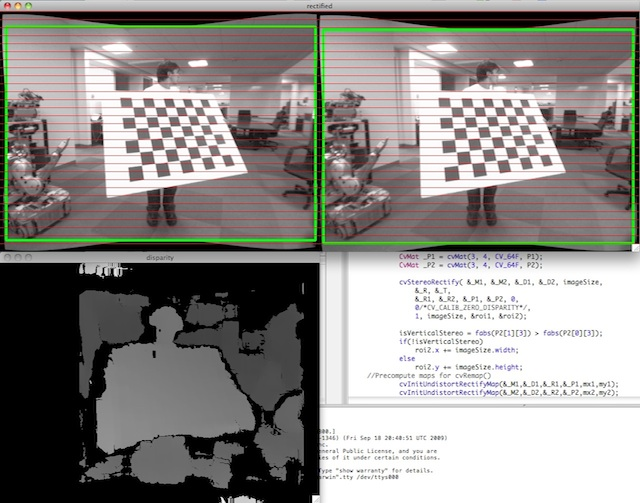
\includegraphics[width=0.8\textwidth]{pics/stereo_undistort.jpg}

\ifCPy
\cvCPyFunc{StereoRectifyUncalibrated}
\else
\cvCppFunc{stereoRectifyUncalibrated}
\fi
Computes rectification transform for uncalibrated stereo camera.

\cvdefC{void cvStereoRectifyUncalibrated( \par const CvMat* points1, \par const CvMat* points2,
                                  \par const CvMat* F, \par CvSize imageSize,
                                  \par CvMat* H1, \par CvMat* H2,
                                  \par double threshold=5 );}
\cvdefPy{StereoRectifyUncalibrated(points1,points2,F,imageSize,H1,H2,threshold=5)-> None}
\cvdefCpp{bool stereoRectifyUncalibrated( const Mat\& points1,\par
                                const Mat\& points2,\par
                                const Mat\& F, Size imgSize,\par
                                Mat\& H1, Mat\& H2,\par
                                double threshold=5 );}
\begin{description}
\cvarg{points1, points2}{The 2 arrays of corresponding 2D points. The same formats as in \cvCross{FindFundamentalMat}{findFundamentalMat} are supported}
\cvarg{F}{The input fundamental matrix. It can be computed from the same set of point pairs using \cvCross{FindFundamentalMat}{findFundamentalMat}.}
\cvarg{imageSize}{Size of the image.}
\cvarg{H1, H2}{The output rectification homography matrices for the first and for the second images.}
\cvarg{threshold}{The optional threshold used to filter out the outliers. If the parameter is greater than zero, then all the point pairs that do not comply the epipolar geometry well enough (that is, the points for which $|\texttt{points2[i]}^T*\texttt{F}*\texttt{points1[i]}|>\texttt{threshold}$) are rejected prior to computing the homographies.
Otherwise all the points are considered inliers.}
\end{description}

The function computes the rectification transformations without knowing intrinsic parameters of the cameras and their relative position in space, hence the suffix "Uncalibrated". Another related difference from \cvCross{StereoRectify}{stereoRectify} is that the function outputs not the rectification transformations in the object (3D) space, but the planar perspective transformations, encoded by the homography matrices \texttt{H1} and \texttt{H2}. The function implements the algorithm \cite{Hartley99}. 

Note that while the algorithm does not need to know the intrinsic parameters of the cameras, it heavily depends on the epipolar geometry. Therefore, if the camera lenses have significant distortion, it would better be corrected before computing the fundamental matrix and calling this function. For example, distortion coefficients can be estimated for each head of stereo camera separately by using \cvCross{CalibrateCamera2}{calibrateCamera} and then the images can be corrected using \cvCross{Undistort2}{undistort}, or just the point coordinates can be corrected with \cvCross{UndistortPoints}{undistortPoints}.


\ifCPy
\cvCPyFunc{Undistort2}
\else
\cvCppFunc{undistort}
\fi
Transforms an image to compensate for lens distortion.

\cvdefC{void cvUndistort2( \par const CvArr* src,\par CvArr* dst,\par const CvMat* cameraMatrix,
    \par const CvMat* distCoeffs, \par const CvMat* newCameraMatrix=0 );}
\cvdefPy{Undistort2(src,dst,cameraMatrix,distCoeffs)-> None}

\cvdefCpp{void undistort( const Mat\& src, Mat\& dst, const Mat\& cameraMatrix,\par
                const Mat\& distCoeffs, const Mat\& newCameraMatrix=Mat() );}
\begin{description}
\cvarg{src}{The input (distorted) image}
\cvarg{dst}{The output (corrected) image; will have the same size and the same type as \texttt{src}}
\cvarg{cameraMatrix}{The input camera matrix $A = \vecthreethree{f_x}{0}{c_x}{0}{f_y}{c_y}{0}{0}{1} $}
\cvarg{distCoeffs}{The input vector of distortion coefficients $(k_1, k_2, p_1, p_2[, k_3[, k_4, k_5, k_6]])$ of 4, 5 or 8 elements. If the vector is NULL/empty, the zero distortion coefficients are assumed.}
\cvCpp{\cvarg{newCameraMatrix}{Camera matrix of the distorted image. By default it is the same as \texttt{cameraMatrix}, but you may additionally scale and shift the result by using some different matrix}}
\end{description}

The function transforms the image to compensate radial and tangential lens distortion.

The function is simply a combination of \cvCross{InitUndistortRectifyMap}{initUndistortRectifyMap} (with unity \texttt{R}) and \cvCross{Remap}{remap} (with bilinear interpolation). See the former function for details of the transformation being performed.

Those pixels in the destination image, for which there is no correspondent pixels in the source image, are filled with 0's (black color).

The particular subset of the source image that will be visible in the corrected image can be regulated by \texttt{newCameraMatrix}. You can use \cvCross{GetOptimalNewCameraMatrix}{getOptimalNewCameraMatrix} to compute the appropriate \texttt{newCameraMatrix}, depending on your requirements.

The camera matrix and the distortion parameters can be determined using
\cvCross{CalibrateCamera2}{calibrateCamera}. If the resolution of images is different from the used at the calibration stage, $f_x, f_y, c_x$ and $c_y$ need to be scaled accordingly, while the distortion coefficients remain the same.


\ifCPy
\cvCPyFunc{UndistortPoints}
\else
\cvCppFunc{undistortPoints}
\fi
Computes the ideal point coordinates from the observed point coordinates.

\cvdefC{void cvUndistortPoints( \par const CvMat* src, \par CvMat* dst,
                        \par const CvMat* cameraMatrix,
                        \par const CvMat* distCoeffs,
                        \par const CvMat* R=NULL,
                        \par const CvMat* P=NULL);}
\cvdefPy{UndistortPoints(src,dst,cameraMatrix,distCoeffs,R=NULL,P=NULL)-> None}

\cvdefCpp{void undistortPoints( const Mat\& src, vector<Point2f>\& dst,\par
                      const Mat\& cameraMatrix, const Mat\& distCoeffs,\par
                      const Mat\& R=Mat(), const Mat\& P=Mat());\newline
void undistortPoints( const Mat\& src, Mat\& dst,\par
                      const Mat\& cameraMatrix, const Mat\& distCoeffs,\par
                      const Mat\& R=Mat(), const Mat\& P=Mat());}

\begin{description}

\cvarg{src}{The observed point coordinates, 1xN or Nx1 2-channel (CV\_32FC2 or CV\_64FC2).} 
\cvarg{dst}{The output ideal point coordinates, after undistortion and reverse perspective transformation\cvCPy{, same format as \texttt{src}}.}
\cvarg{cameraMatrix}{The camera matrix $\vecthreethree{f_x}{0}{c_x}{0}{f_y}{c_y}{0}{0}{1}$}
\cvarg{distCoeffs}\cvarg{distCoeffs}{The input vector of distortion coefficients $(k_1, k_2, p_1, p_2[, k_3[, k_4, k_5, k_6]])$ of 4, 5 or 8 elements. If the vector is NULL/empty, the zero distortion coefficients are assumed.}
\cvarg{R}{The rectification transformation in object space (3x3 matrix). \texttt{R1} or \texttt{R2}, computed by \cvCppCross{StereoRectify} can be passed here. If the matrix is empty, the identity transformation is used}
\cvarg{P}{The new camera matrix (3x3) or the new projection matrix (3x4). \texttt{P1} or \texttt{P2}, computed by \cvCppCross{StereoRectify} can be passed here. If the matrix is empty, the identity new camera matrix is used}
\end{description}

The function is similar to \cvCross{Undistort2}{undistort} and \cvCross{InitUndistortRectifyMap}{initUndistortRectifyMap}, but it operates on a sparse set of points instead of a raster image. Also the function does some kind of reverse transformation to \cvCross{ProjectPoints2}{projectPoints} (in the case of 3D object it will not reconstruct its 3D coordinates, of course; but for a planar object it will, up to a translation vector, if the proper \texttt{R} is specified).

\begin{lstlisting}
// (u,v) is the input point, (u', v') is the output point
// camera_matrix=[fx 0 cx; 0 fy cy; 0 0 1]
// P=[fx' 0 cx' tx; 0 fy' cy' ty; 0 0 1 tz]
x" = (u - cx)/fx
y" = (v - cy)/fy
(x',y') = undistort(x",y",dist_coeffs)
[X,Y,W]T = R*[x' y' 1]T
x = X/W, y = Y/W
u' = x*fx' + cx'
v' = y*fy' + cy',
\end{lstlisting}

where undistort() is approximate iterative algorithm that estimates the normalized original point coordinates out of the normalized distorted point coordinates ("normalized" means that the coordinates do not depend on the camera matrix).

The function can be used both for a stereo camera head or for monocular camera (when R is \cvC{NULL}\cvPy{None}\cvCpp{empty}).
